\documentclass[aos,preprint]{imsart}
\usepackage{xr}
	\externaldocument{./suppl}

%% Packages
\def\shownotes{1}
%\usepackage{natbib}
%\setcitestyle{authoryear,open={(},close={)}}
%\renewcommand{\cite}{\citep}
\usepackage[export]{adjustbox}
%\usepackage[margin=1in]{geometry}
%\usepackage{fullpage}
\usepackage{subfloat}
\usepackage[T1]{fontenc}    % use 8-bit T1 fonts
\usepackage{nicefrac}       % compact symbols for 1/2, etc.
\usepackage{microtype}      % microtypography
\usepackage{graphicx}
\usepackage[hidelinks]{hyperref}
\usepackage{macro_math}
\usepackage{macro_fan}
\usepackage{stmaryrd}
\usepackage{multirow}
\usepackage[us,12hr]{datetime}
\usepackage[utf8]{inputenc} % allow utf-8 input
\usepackage{caption,subcaption}
%\usepackage{breqn}

\usepackage{dsfont}


\newcommand*\samethanks[1][\value{footnote}]{\footnotemark[#1]}

\endlocaldefs

\begin{document}

\begin{frontmatter}

\title{High-dimensional Asymptotics of Information Transfer for Linear Regression under Covariate Shifts}

\runtitle{High-dimensional Asymptotics of Information Transfer}
%\thankstext{T1}{A sample additional note to the title.}

\begin{aug}
%%%%%%%%%%%%%%%%%%%%%%%%%%%%%%%%%%%%%%%%%%%%%%
%%Only one address is permitted per author. %%
%%Only division, organization and e-mail is %%
%%included in the address.                  %%
%%Additional information can be included in %%
%%the Acknowledgments section if necessary. %%
%%%%%%%%%%%%%%%%%%%%%%%%%%%%%%%%%%%%%%%%%%%%%%
\author[A]{\fnms{Fan} \snm{Yang}\ead[label=e1]{}},
\author[B]{\fnms{Hongyang R.} \snm{Zhang}\ead[label=e2]{}},
\author[C]{\fnms{Sen} \snm{Wu}\ead[label=e3]{}},\\
\author[A]{\fnms{Weijie J.} \snm{Su}\ead[label=e4]{} },
\and
\author[C]{\fnms{Christopher} \snm{R\'e}\ead[label=e5]{}}
%%%%%%%%%%%%%%%%%%%%%%%%%%%%%%%%%%%%%%%%%%%%%%
%% Addresses                                %%
%%%%%%%%%%%%%%%%%%%%%%%%%%%%%%%%%%%%%%%%%%%%%%
\address{${ }^{1}$University of Pennsylvania, ${ }^{2}$Northeastern University, ${ }^{3}$Stanford University
}
%}\address[C]{
%}

\end{aug}

% The idea is to use a shared feature space for all tasks, while each task also has a separate layer for making the prediction.
\begin{abstract}
	Hard parameter sharing for multi-task learning is widely used in empirical research despite the fact that their generalization properties have not been established in many cases. This paper studies a fundamental question to better understand this approach: How does hard parameter sharing work given multiple linear regression tasks? We develop new techniques and establish a number of new results in the high-dimensional setting, where the sample size and feature dimension become increasingly large in a fixed ratio. First, we show a sharp bias-variance decomposition of hard parameter sharing, given multiple tasks with the same features. Second, we characterize the asymptotic bias-variance limit for two tasks, even when they have arbitrarily different sample size ratios and covariate shifts. We also demonstrate that these limiting estimates for the empirical loss are incredibly accurate in moderate dimensions. Finally, we explain an intriguing phenomenon where increasing one task's sample size helps another task initially by reducing variance but hurts eventually due to increasing bias. This suggests progressively adding data for optimizing hard parameter sharing, and we validate its efficiency in text classification tasks.
\end{abstract}

\section{Introduction}\label{sec introduction}

\iffalse
%Multi-task learning is an inductive learning mechanism to improve generalization performance using related task data.
%Many state-of-the-art results in computer vision and natural language processing are obtained using multi-task learning.
Multi-task learning is a powerful approach to improve performance for many tasks in computer vision, natural language processing, and other areas \cite{C97,ZY17,R17}.
%In multi-task learning, having related task data is fundamental to its performance.
%Multi-task learning is particularly powerful when there is limited labeled data for a task to be solved, meanwhile more labeled data from different but related tasks is available.
%By combining multiple information sources, it is possible to share all the information in the same model.
In many settings, multiple source tasks are available to help with predicting a particular target task.
\todo{clarify setting is different from traditional MTL}
%For example, many applications in , and many other areas have been achieved by learning from multiple tasks together.
The performance of multi-task learning depends on the relationship between the source and target tasks \cite{C97}.
%	We define that multi-task learning provides \textit{positive transfer} if it outperforms single-task learning, or \textit{negative transfer} otherwise.
When the sources are relatively different from the target, multi-task learning (MTL) has often been observed to perform worse than single-task learning (STL) \cite{AP16,BS17}, which is referred to as \textit{negative transfer} \cite{PY09}.
While many empirical approaches have been proposed to mitigate negative transfer \cite{ZY17}, a precise understanding of when negative transfer occurs remains elusive in the literature \cite{R17}.
%This phenomenon, known as \textit{negative transfer}, is fundamental to the understanding of multi-task learning.

%Inspired by the theory, we propose an incremental training schedule to improve multi-task training.
%We consider a setting where the target task has limited labeled data and show
%On the other hand, unless the structures across task data are well-understood, applying multi-task learning on several different datasets often result in suboptimal models (or negative transfer in more technical terms).

Understanding negative transfer requires developing generalization bounds that scale tightly with properties of each task data, such as its sample size.
This presents a technical challenge in the multi-task setting because of the difference among task features, even for two tasks.
ithout a tight lower bound for multi-task learning, comparing its performance to single-task learning results in vacuous bounds.
\todo{add more technical motivation (or maybe later)}
From a practical standpoint, developing a better understanding of multi-task learning in terms of properties of task data can provide guidance for downstream applications \cite{RH19}.
%For example,
%On the other hand, uneven sample sizes (or dominating tasks) have been empirically observed to cause negative transfer \cite{YKGLHF20}.
%The benefit of learning multi-task representations has also been studied for certain half-spaces \cite{} and sparse regression \cite{}.
%When all tasks are sufficiently similar, adding more labeled data improves the generalization performance for predicting a particular task \cite{WZR20}.

%\textbf{Setup and Main Results.}
In this work, we study the bias and variance of multi-task learning in the high-dimensional linear regression setting \cite{HMRT19,BLLT20}.
Our key observation is that three properties of task data, including \textit{task similarity}, \textit{sample ratio}, and \textit{covariate shift}, can affect whether multi-task learning outperforms single-task learning (which we refer to as \textit{positive transfer}).
As an example, we vary each property in Figure \ref{fig_model_shift_phasetrans} for two linear regression tasks and measure the improvement of multi-task learning over single-task learning for a particular task.
We observe that the effect of transfer can be either positive or negative as we vary each property.
These phenomena cannot be explained using previous techniques \cite{WZR20}.
The high-dimensional linear regression setting allows us to measure the three properties precisely.
Here we define each property for the case of two tasks, while our definition applies to general settings.
We refer to the first task as the source task and the second as the target task.
\squishlist
	\item \textbf{Task similarity:} Assume that both tasks follow a linear model with parameters $\beta_1, \beta_2\in\real^p$, respectively.
	We measure the distance between them by $\norm{\beta_1 - \beta_2}$.
	\item \textbf{Sample ratio:} Let $n_1 = \rho_1 \cdot p, n_2 = \rho_2 \cdot p$ be the sample size of each task, where $\rho_1, \rho_2>1$ are both fixed values that do not grow with $p$.
	We measure the source/target sample ratio by $\rho_1 / \rho_2$.
%	Importantly, $\rho_2$ can be a small constant (say $2$) to capture the need for more labeled data.
	\item \textbf{Covariate shift:} Assume that the task features are random vectors with positive semidefinite covariance matrices $\Sigma_1\in\real^{p\times p}$ and $\Sigma_2\in\real^{p\times p}$, respectively.
	%$x = \Sigma_i^{1/2}z$, where $z\in\real^p$ consists of i.i.d. entries with mean zero and unit variance, and is a positive semidefinite matrix.
	We measure covariate shift with matrix $\Sigma_1^{1/2}\Sigma_2^{-1/2}$.
\squishend
\fi


Hard parameter sharing (HPS) for multi-task learning is widely used in empirical research and goes back to the seminal work of \citet{C97}.
Recent work has revived interest in this approach because it improves performance and reduces the cost of collecting labeled data \cite{MTDNN19,ZSSGM18}.
It is generally applied by sharing the feature layers between all tasks while keeping an output layer for every task.
Often, hard parameter sharing offers two critical advantages if successfully applied.
(i) It reduces model parameters since all tasks use the same feature space.
(ii) It reduces the amount of labeled data needed from each task by augmenting the entire training dataset.

Hard parameter sharing offers great intuitive appeal as an inductive transfer mechanism.
It reduces overfitting by acting as a regularizer \cite{R17}.
For example, by restricting the shared space's size, HPS encourages information sharing among multiple tasks \cite{KD12}.
Another source of inductive bias comes from the tasks and depends on datasets' properties such as sample sizes and task covariances \cite{WZR20}.
However, how these dataset properties impacts HPS has not been established.
%It becomes increasingly important to understand HPS' formal generalization properties.
Part of the challenge may be that HPS' generalization performance depends intricately on the sample size ratios and covariate shifts between tasks, not amenable to standard concentration results.
Previous results based on Rademacher complexity or VC dimensions have considered when all tasks' sample sizes are equal to logarithm factors of feature dimension \cite{B00,MPR16}, and when all tasks' sample sizes increase simultaneously \cite{AZ05,M06}.
%For, the generalization error scales down as the sample sizes of all tasks increase, when applied to the multi-task setting \cite{B00,AZ05,M06,MPR16,WZR20}.

This paper presents new techniques to study hard parameter sharing and establish a number of new results.
We consider regression analysis, which is arguably one of the most fundamental problems in statistics and machine learning.
We are interested in the \textit{high-dimensional} setting, where each dataset's sample size and feature dimension grow linearly at a fixed ratio.
This is motivated by many multi-task learning applications, where the amount of labeled data from each dataset is usually insufficient for learning a single task.
For example, this is the case if a dataset's sample size is only a small constant factor of the feature dimension.
The high-dimensional setting is challenging but is crucial for understanding how datasets' sample sizes impact generalization performance.


\medskip
\noindent\textbf{Notations.}
%Let $\cE \define [\varepsilon_1, \varepsilon_2, \dots, \varepsilon_t] \in \real^{n \times t}$ denote the random noise.
%We can also write $Y = XB^{\star} + \cE$.
%Let $A = [A_1, A_2, \dots, A_t] \in \real^{r\times t}$ be a matrix notation that contains all the output layer parameters.
For an $n\times p$ matrix $X$, let $\lambda_{\min}(X)$ denote its smallest singular value and $\norm{X}$ denote its largest singular value.
Let $\lambda_1(X), \lambda_2(X), \cdots, \lambda_{p\wedge n}(X)$ denote the singular values of $X$ in decreasing order.
Let $X^+$ denote the Moore-Penrose psuedoinverse of $X$.
We refer to random matrices of the form $\frac {X^\top X} n$ as sample covariance matrices.
We say that an event $\Xi$ holds with high probability if the probability that $\Xi$ happens goes to $1$ as $p$ goes to infinity.
We use the big-O notation $g(n) = \OO(f(n))$ if there exists a constant $C$ such that $g(n) \le C \dot f(n)$ for large enough $n$. Moreover, we use the notation $g(n)\lesssim f(n)$ if $g(n) = \OO(f(n))$, and the notation $g(n)\sim f(n)$ if $g(n) \lesssim f(n))$ and $f(n) \lesssim g(n)$. In this paper, we will often write an identity matrix $\id_{n\times n}$ as $1$ without causing any confusions. 
%We shall use $\oo(1)$ to mean a small positive quantity that converges to 0 as $p$ goes to infinity.


\section{High-dimensional asymtotics of information transfer}\label{sec_HPS}
In this section, we define our model for the setting of transfer learning, and introduce several transfer learning estimators that will be considered in this paper. 


\subsection{Assumptions}
Furthermore, we assume that the entries $z^{(1)}_{ij}$ and $z^{(2)}_{ij}$ have finite $\varphi$-th moment for some constant $\varphi>4$:
\be \label{conditionA2}
\mathbb{E} \vert z^{(1)}_{ij} \vert^\varphi  \le \tau^{-1},\quad \mathbb{E} \vert  z^{(2)}_{ij} \vert^\varphi   \le \tau^{-1}
\ee
for a small constant $\tau>0$. We assume that $\Sig^{(i)}$ has eigendecomposition
\be\label{eigen}
\Sig^{(i)}= O_i\Lambda_i O_i^\top, \quad  \Lambda_1=\text{diag}(\si_1^{(i)}, \ldots, \si^{(i)}_n),  \quad i=1,2,
\ee
where $O_i$ is the eigenmatrix and the eigenvalues satisfy that
\begin{equation}\label{assm3}
 \tau \le  \si^{(i)}_p \le\cdots\le \si^{(i)}_2 \le \si^{(i)}_1 \le \tau^{-1} \quad i=1,2.
\ee
%for a small constant $\tau>0$. 

We assume that $\varepsilon^{(1)} \in \real^{n}$ and $\varepsilon^{(2)} \in \real^{n}$ are two independent random noise vectors with i.i.d entries of mean zero, variance $\sigma^2$, and bounded moment up to any order: for any fixed $k\in \N$, there exists a constant $C_k>0$ such that 
\be\label{eq_highmoments}
\E  | \ve^{(1)}_{i} |^k \le C_k,\quad \E  | \ve^{(2)}_{i} |^k \le C_k.
\ee
Finally, we assume that $\beta^{(1)}$ and $\beta^{(2)}$ are two arbitrary deterministic or random vectors that are independent of $X^{(1)}$, $X^{(2)}$, $\varepsilon^{(1)}$ and $\varepsilon^{(2)}$. 
%Moreover, we assume that 
%\be\label{eq_SNR}
%\tau\le \frac{\|\beta^{(1)}\|^2}{\|\beta^{(2)}\|^2} \le \tau^{-1},\quad  \frac{\|\beta^{(1)}\|^2}{\sigma^2} \ge \tau,
%\ee
%for a small constant $\tau >0$. The first condition means that the norms of the two model parameters $\beta^{(1)}$ and $\beta^{(2)}$ are comparable, while the second condition means that the singal-to-noise ratio cannot be too small.
 
In this paper, we consider the high-dimensional setting, where the sample ratios satisfy that  %We assume that the aspect ratios $d_1:= p/n_1$ and $d_2:=p/n_2$ satisfy that 
\be\label{assm2}
1+\tau \le \rho_1:=\frac{n_1}{p} \le p^{\tau^{-1}}, \quad 1+\tau \le \rho_2:=\frac{n_2}{p} \le p^{\tau^{-1}}, \quad \tau \le \frac{\rho_1}{\rho_2}\le \tau^{-1},
\ee
for a small constant $\tau >0$. If $\rho_i>p^{\tau^{-1}}$, $i=1,2$, we are basically in the low-dimensional region, where the law of large numbers and central limit theorem already  give good enough results without using the theory developed in this paper. The lower bounds $\rho_1> 1+\tau$ and ${\rho_2 > 1+ \tau}$ 
are to ensure that the sample covariance matrices $  (X^{(1)})^\top X^{(1)} $ and $  (X^{(2)})^\top X^{(2)} $ are non-singular with high probability, so that the ordinary least squares (OLS) estimator is well-defined for the linear regression problem on each task.  


We summarize our basic assumptions here for future reference.
\begin{assumption}\label{assm_big1}
Let $\tau$ be a small constant. 
\begin{enumerate}
\item  $X^{(1)}$ and $X^{(2)}$ take the form \eqref{XofZ}, where $Z^{(1)}$ and $Z^{(2)}$ are respectively $n_1\times p$ and $n_2\times p$ random matrices with i.i.d. entries satisfying (\ref{assm1}) and \eqref{conditionA2}, $\Sig^{(1)}$ and $\Sig^{(2)}$ are deterministic positive definite symmetric matrices satisfying \eqref{eigen} and \eqref{assm3}. %and (\ref{assm2}). We assume that $T$ is an $M\times M$ deterministic diagonal matrix satisfying (\ref{simple_assumption}) and (\ref{assm3}).  
 
\item $\varepsilon^{(1)} \in \real^{n}$ and $\varepsilon^{(2)} \in \real^{n}$ are random vectors independent from $X^{(1)}$ and $X^{(2)}$, and with i.i.d entries of mean zero, variance $\sigma^2$, and bounded moments as in \eqref{eq_highmoments}.  

\item $\beta^{(1)}$ and $\beta^{(2)} $ are independent of $X^{(1)}$, $X^{(2)}$, $\varepsilon^{(1)}$ and $\varepsilon^{(2)} $. %, and satisfy \eqref{eq_SNR}. 
 
\item $\rho_{1}$ and $\rho_{2}$ satisfy \eqref{assm2}.

\end{enumerate}
\end{assumption}
 
%\subsection{Transfer learning estimators}


%\FY{Introduce some popular transfer learning estimators: total loss estimator, and model averaging estimator.}


In this paper, we measure the performance of $\hat{\beta}_2^{\MTL} (\hat a)$ through the out-of-sample predication loss (test error). Consider a test data point $(x,y)$ generated from the same model as task 2: $y= x^\top \beta^{(2)} + \ve$, where $x \in \R^p$ and $\ve\in \R$ are independent of $X^{(1)}$, $X^{(2)}$, $\varepsilon^{(1)}$ and $\varepsilon^{(2)}$, and only $x$ is observable. We want to use $x^\top \hat{\beta}_2^{\MTL} (\hat a) $ to predict $y$, and we measure the predication loss using the mean squared error
$$\exarg{x}{\left\|y-x^\top \hat{\beta}_2^{\MTL} (\hat a) \right\|^2}= \left\|(\Sigma^{(2)})^{1/2} \left(\hat{\beta}_2^{\MTL} (\hat a)  - \beta^{(2)}\right)\right\|^2 + \sigma^2.  $$ 
Since $\sigma^2$ is a constant that does not depend on the model, we ignore it and define the predication loss as
\be\label{HPS_loss}
L(\hat{\beta}_2^{\MTL}(\hat a)):= \left\|(\Sigma^{(2)})^{1/2} \left(\hat{\beta}_2^{\MTL} (\hat a)  - \beta^{(2)}\right)\right\|^2 .
 \ee
We will compare it to the out-of-sample predication losses of the baseline estimators, $L(\hat{\beta}_2^{\STL})$ and $L(\hat{\beta}^{\AV}(\lambda))$ for some properly chosen $\lambda\in [0,1]$. 

%$L(\hat{\beta}_2^{\STL})$ of the single-task OLS estimator  as a baseline.  

Plugging \eqref{HPS_est} into \eqref{HPS_loss}, we get
\begin{align}
L(\hat{\beta}_2^{\MTL}(\hat a))  =  &\left\| (\Sigma^{(2)})^{1/2}\hat \Sigma(\hat a)^{-1} (X^{(1)})^\top X^{(1)} (\hat a\beta^{(1)}-\hat a^2\beta^{(2)}) \right. \nonumber\\
&\left. +(\Sigma^{(2)})^{1/2}\hat \Sigma(\hat a)^{-1} \left[ (X^{(2)})^\top \epsilon^{(2)} + \hat a  (X^{(1)})^\top \epsilon^{(1)} \right]\right\|^2.\label{Lbeta_HPS}
\end{align}
Note that if we replace $\hat a$ with a fixed number $a$ in \eqref{Lbeta_HPS}, then taking the expectation over $\ve^{(1)}$ and $\ve^{(2)}$, we can get a clean bias-variance decomposition of the predication loss:
\be\label{partial-L} \exarg{\ve^{(1)},\ve^{(2)}}{L(\hat{\beta}_2^{\MTL}(a)) } = L_{\bias} (a) + L_{\var}(a),\ee
where 
\be\label{Lbias} L_{\bias} (a) := \left\| (\Sigma^{(2)})^{1/2}\hat \Sigma(a)^{-1} (X^{(1)})^\top X^{(1)} \left(a\beta^{(1)}- a^2\beta^{(2)}\right) \right\|^2 \ee
is called the bias term, which depends on the model bias between task 1 and task 2, and
\be\label{Lvar}  L_{\var}(a):=\sigma^2  \bigtr{{\Sigma^{(2)}\hat \Sigma(a)^{-1}  }} \ee
is called the variance term, which depends on the noise variance. Using concentration of the noise vectors $\ve^{(1)}$ and $\ve^{(2)}$, we can show that $L(\hat{\beta}_2^{\MTL}(a))$ is close to \eqref{partial-L} up to a small error as in the next lemma. In this paper, we say that an event $\Xi$ holds \emph{with high probability} (w.h.p.) if $\mathbb P(\Xi)\to 1$ as $p\to \infty$.
%predication loss for the HPS and OLS estimators. 

 
 \begin{lemma}\label{lem_HPS_loss}
 Under Assumption \ref{assm_big1}, for any small constant $\e>0$ and large constant $C>0$, there exists a high probability event $\Xi$, on which the following estimates hold uniformly in $a\in \R$ and $\lambda\in [0,1]$: 
\begin{align}
L(\hat{\beta}_2^{\MTL}(a)) &=\left[ 1+ \OO(p^{-1/2+c})\right]\cdot \left[L_{\bias} (a) + L_{\var}(a)\right] \nonumber\\
&+ \OO \left[ p^{-C}\left( \|\beta^{(1)} \|^2  +  \|\beta^{(2)} \|^2\right)   \right], \label{L_HPS_simple}
\end{align}
\begin{align}
L(\hat{\beta}^{\AV}(\lambda) ) &= \left[ 1+ \OO(p^{-1/2+c})\right] \cdot \lambda^2 \left\| (\Sigma^{(2)})^{1/2}(\beta^{(1)}-\beta^{(2)})\right\|^2 \nonumber \\
&+  \left[ 1+ \OO(p^{-1/2+c})\right] \cdot \sigma^2   \lambda^2 \bigtr{\Sigma^{(2)} [(X^{(1)})^\top X^{(1)}]^{-1}  }\nonumber\\
& + \left[ 1+ \OO(p^{-1/2+c})\right] \cdot \sigma^2  (1-\lambda)^2 \bigtr{\Sigma^{(2)} [(X^{(2)})^\top X^{(2)}]^{-1}  }  . \label{L_AVE_simple}
\end{align}
and 
\begin{align}
L(\hat{\beta}_2^{\STL} ) &= \left[ 1+ \OO(p^{-1/2+c})\right] \cdot \sigma^2  \bigtr{\Sigma^{(2)} [(X^{(2)})^\top X^{(2)}]^{-1}  }  . \label{L_STL_simple}
\end{align}
%Moreover, there exists a constant $C_0>0$ such that with high probability,
%\be\label{loss_large}
%g(a) > g(0) \quad \text{for all $a$ such that }|a|\ge C_0.
%\ee
%with high probability for any small constant $\e>0$. 
\end{lemma}

 

Since \eqref{L_HPS_simple} holds uniformly for all $a\in \R$, we can also apply it to $\hat{\beta}_2^{\MTL}(\hat a)$, where $\hat a$ is a random variable that may depend on $\ve^{(1)}$ and $\ve^{(2)}$. In practice, the parameter $ a$  is up to one's choice and may not be the global minimizer, so we have stated the result for an completely arbitrary $a$. (In fact, the optimization objective $g(a)$ is generally non-convex, so in some cases one can only find a local minimizer.) For a fixed $a\in \R$, the proof of \eqref{L_HPS_simple} is based on the sharp concentration bounds in Lemma \ref{largedeviation} of the supplement \cite{MTL_suppl}. To extend uniformly to all $a\in \R$, we will use a standard $\ve$-net argument, which leads to a small error $ p^{-C}\left( \|\beta^{(1)} \|^2  +  \|\beta^{(2)} \|^2\right) $. Note that this error is negligible unless $\beta^{(1)}$ and $ a\beta^{(2)}$ cancel each other almost exactly, and the noise variance $\sigma$ is very small. The proof of Lemma \ref{lem_HPS_loss} will be given in Appendix  \ref{app_firstpf} of the supplement \cite{MTL_suppl}. 

%In this section, we show that the prediction loss of hard parameter sharing admits a clean bias-variance decomposition, when all tasks have the same features.




For the single-task predication loss \eqref{L_STL_simple}, we can calculate its asymptotic limit exactly using the following classical result in multivariate statistics.
 
\begin{lemma}[Theorem 2.4 of \cite{isotropic} and Theorem 3.14 of \cite{DY}]\label{fact_tr}
	%Let $X  \in \real^{n\times p}$ be a random matrix that satisfies Assumption \ref{assume_rm}.
	%Let $\Sigma\in\real^{p\times p}$ denote the population covariance matrix of $X$.
	Under Assumption \ref{assm_big1}, we have that for any deterministic $p\times p$ matrix $\Sigma$,
		\[ \bigtr{\Sigma \frac1{(X^{(2)})^\top X^{(2)} }  } %= \bigtr{ \frac1{(Z^{(2)})^\top Z^{(2)} }  } 
		= \frac{1}{n_2 - p}\bigtr{\Sigma (\Sigma^{(2)})^{-1}} +  \OO\left( \frac{p^{\e}}{\sqrt{n_2 p}}\cdot \frac{p}{n_2}\|A\| \right) \]
		with high probability for any small constant $\e>0$.
\end{lemma}
 %The above result has a long history in random matrix theory.
If the entries of $Z^{(2)}$ are i.i.d. Gaussian, then this result follows from the classical result for %the mean of 
the inverse Wishart distribution \cite{anderson1958introduction}. For a general non-Gaussian $Z^{(2)}$, this result can be obtained using the well-known Stieltjes transform method (cf. Lemma 3.11 of \cite{bai2009spectral}). Here we have presented the results from \cite{isotropic,DY}, which give an almost sharp convergence rate. With Lemma \ref{fact_tr}, we obtain that w.h.p.,
\begin{align}
L(\hat{\beta}_2^{\STL} ) &= \left[ 1+ \OO(p^{-1/2+c})\right] \cdot \frac{p \sigma^2 }{n_2-p}   , \label{L_STL_simple01}
\end{align}
and
\begin{align}
L(\hat{\beta}^{\AV}(\lambda) ) &= \left[ 1+ \OO(p^{-1/2+c})\right] \cdot \lambda^2 \left\| (\Sigma^{(2)})^{1/2}(\beta^{(1)}-\beta^{(2)})\right\|^2 \nonumber \\
&+  \left[ 1+ \OO(p^{-1/2+c})\right] \cdot \sigma^2 \left[\frac{ \lambda^2}{n_1-p}\bigtr{\Sigma^{(2)}(\Sigma^{(1)})^{-1}} + \frac{(1-\lambda)^2p  }{n_2-p}\right] . \label{L_AVE_simple01}
 \end{align}

On the other hand, much less is known about the predication loss of the HPS estimator. In particular, its exact dependence on the model parameters, including the model bias, noise variance, sample sizes, and population covariance matrices, is not well-understood so far. %\FY{What is known so far about this topic?} 
In Section \ref{sec_HPS_loss}, we give a rigorous analysis of the bias term \eqref{Lbias} and variance term \eqref{Lvar} in two different settings: (i) independent $X^{(1)}$ and $X^{(2)}$ with different sample sizes and same population covariance matrices $\Sigma^{(1)}=\Sigma^{(2)}$; (ii) independent $X^{(1)}$ and $X^{(2)}$ with different sample sizes and different population covariance matrices. In case (i), we provide the exact asymptotics for both the bias and variance terms, together with almost sharp convergence rates. We will use these results to illustrate the effects of the \emph{bias-variance tradeoff} and \emph{varying sample sizes}. In case (ii), we will prove an exact asymptotic variance limit, and employ the result to show the intricate effect of the covariate shift. On the other hand, in case (ii), we will provide an estimate on the bias term, which becomes exact only when $n_1\gg p$. %Here case (ii) is actually more general than (i) 
%In particular, we will use our results to analyze the effect of the following factors: \emph{bias-variance tradeoff}, \emph{sample sizes}, and \emph{covariate shift}.   
In Section \ref{sec_same}, we will consider a simple extension to a multi-task learning setting with more than two tasks and  the same covariates for all tasks. We will give the asymptotic limit of the predication loss for the HPS estimator, which provides useful insights into the more rich multi-task learning theory. Due to length constraint, we will explore the multi-task learning setting in greater details in other works.

%{\cor discuss about the bias-variance trade-off}
%However, to the best of our knowledge, the asymptotic limit of $L(\hat{\beta}_2^{\MTL}(a))$ has never been calculated exactly in any high-dimensional setting. 

  
%\section{Predication loss for HPS estimator}\label{sec_HPS_loss}
	

	
\subsection{Covariate shift}\label{sec_diff}

%The previous section assumes that all tasks have the same sample size and feature vectors.
In this section, we consider the most general setting, where the feature covariates $X^{(1)}$ and $X^{(2)}$ of the two tasks have both different sample sizes and different population covariance matrices.
%The different covariates case differs from the same covariates case in two aspects.
%First, different tasks may have different sample sizes. In extreme scenarios, one task may have much less labeled data compared to another task.
In particular, the fact that population covariance matrices differ across tasks is often called ``covariate shift''. %which is characterized by the matrix $(\Sigma^{(1)})^{1/2}(\Sigma^{(2)})^{-1/2}$. 
In this section, we describe the exact asymptotic variance limit in the high-dimensional setting, while the bias limit is much more complicated, and we can only give an estimate on it.

\iffalse
Unlike the previous section, we can no longer characterize the global minimum of $f(A, B)$.
This is because $f(A, B)$ is in general non-convex.
Instead, our result implies sharp bias-variance tradeoffs for any \emph{local minimizer} of $f(A, B)$.
We focus on the two-task case to better understand the impact of having different sample sizes and different covariates.
Let $n_1, n_2$ denote task one  and two's sample size, respectively.
Suppose
\begin{align*}
	X^{(1)} = Z^{(1)}(\Sigma^{(1)})^{1/2} \in \real^{n_1 \times p} \text{ and }
	X^{(2)} = Z^{(2)}(\Sigma^{(2)})^{1/2} \in \real^{n_2 \times p},
\end{align*}
where the entries of $Z^{(1)}$ and $ Z^{(2)}$ are drawn independently from a one dimensional distribution with zero mean, unit variance, and constant $\varphi$-th moment for a fixed $\varphi > 4$. $\Sigma^{(1)}\in \R^{p\times p}$ and $\Sigma^{(2)}\in \R^{p\times p}$ denote the population covariance matrices of task 1 and task 2, respectively.


Without loss of generality, we consider task two's prediction loss and the same result applies to task one.
We consider the case of $r = 1 < t = 2$, since when $r > 1$, the global minimum of $f(A, B)$ reduces to single-task learning (cf. Proposition 1 of \cite{WZR20}).
When $r = 1$, $B$ is a vector and $A_1, A_2$ are both scalars.
To motivate our study, we consider a special case where $A_1=A_2=1$.
Hence the HPS estimator is equal to $B$.
%Hence we can write down a closed form equation for any local minimizer of $f(A, B)$.
By solving $B$ in equation \eqref{eq_mtl}, we obtain the estimator for task two as follows:
\begin{align}
	\hat{\beta}_2^{\MTL} = {\hat{\Sigma}}^{-1} ({X^{(1)}}^{\top} Y^{(1)} + {X^{(2)}}^{\top} Y^{(2)}), \text{ where }
	\hat{\Sigma} = {X^{(1)}}^{\top} X^{(1)} + {X^{(2)}}^{\top} X^{(2)}. \label{def hatsig}
\end{align}
The matrix $\hat{\Sigma}$ adds up both tasks' sample covariance matrices, and the expectation of $\hat{\Sigma}$ is equal to a mixture of their population covariance matrices, with mixing proportions determined by their sample sizes.

To derive the bias and variance equation, we consider the expected loss conditional on the covariates as follows (the empirical loss is close to this expectation as will be shown in equation \eqref{claim_largedev2}):
 %similar to Claim \ref{claim_pred_err}
\begin{align}
	 \exarg{\cE}{L(\hat{\beta}_2^{\MTL}) \mid X^{(1)}, X^{(2)}}
	=& \bignorm{{\Sigma^{(2)}}^{1/2} \hat{\Sigma}^{-1} {X^{(1)}}^{\top} X^{(1)} (\beta^{(1)} - \beta^{(2)})}^2 \label{eq_bias_2task} \\
	& + \sigma^2 \bigtr{\Sigma^{(2)}\hat{\Sigma}^{-1}}. \label{eq_variance_2task}
\end{align}
Equations \eqref{eq_bias_2task} and \eqref{eq_variance_2task} correspond to the bias and variance of HPS for two tasks, respectively.
\fi

%Our key result characterizes the asymptotic limit of the inverse of the sum of two arbitrarily different sample covariance matrices.
Compared to the results in Section \ref{sec_sizeratio}, the spectrum of $\hat{\Sigma}(a)^{-1}$ now not only depends on the sample sizes of both tasks, but also depends on the ``misalignment'' between $\Sigma^{(1)}$ and $\Sigma^{(2)}$. 
%However, capturing this intuition quantitatively turns out to be technically challenging.
%The main technical challenge of our result deals with the ``covariate shift'' between tasks one and two.
To capture this misalignment quantitatively, we introduce the covariate shift matrix %(rescaled by $a$) 
$$ M(a) \define a(\Sigma^{(1)})^{1/2}(\Sigma^{(2)})^{-1/2}.$$ 
%Let $U\Lambda V^\top$ denote the SVD of $M$ and
Let $\lambda_1(a)\ge \lambda_2(a)\ge \dots\ge \lambda_p(a)$ be the singular values of $M$ in descending order. By \eqref{assm3}, these singular values satisfy that
\begin{equation}\label{assm32}
|a| \tau \le  \lambda_p(a) \le \cdots \le \lambda_2(a)\le \lambda_1(a) \le |a|\tau^{-1}. %, \quad \max\left\{\pi_A^{(n)}([0,\tau]), \pi_B^{(n)}([0,\tau])\right\} \le 1 - \tau .
\end{equation}
%for some small constant $0<\tau<1$. 
The main result of this section is the following theorem on the variance limit, which characterizes  the exact dependence of $L_{\var}(a)$ on the singular values of $M$.


\begin{theorem}\label{thm_main_RMT}
%	Let $c_{\varphi}$ be any fixed value within $(0, \frac{\varphi - 4}{2\varphi})$.
%	Assume that: a) the sample sizes $n_1$ and $n_2$ both satisfy Assumption \ref{assume_rm};
%	b) $M$'s singular values are all greater than $\tau$ and less than $1/\tau$;
%	c) task one's sample size is greater than $\tau p$ and task two's sample size is greater than $(1 + \tau) p$.
%	With high probability over the randomness of $X^{(1)}$ and $X^{(2)}$, we have the following limits:
Under Assumption \ref{assm_big1}, for any small constant $c>0$, there exists a high probability event $\Xi$, on which the following estimate holds for $L_{\var}(a)$ in \eqref{Lvar}: 
%equation \eqref{eq_variance_2task} $\tr[\Sigma^{(2)} \hat{\Sigma}^{-1}]$ (leaving out $\sigma^2$) satisfies the following estimate:
			\begin{align}\label{lem_cov_shift_eq}
				\bigabs{L_{\var}(a)- \frac{\sigma^2}{n_1+n_2}\bigtr{  \frac{1}{a_1 M(a)^\top M(a) + a_2  }  }}
				\le \frac{(n_1+n_2)^{2/\varphi + c}}{p^{1/2} (n_1+n_2)^{1/2}}\cdot\frac{p \sigma^2}{n_1+ n_2}  ,
			\end{align}
			 uniformly in all $a\in \R$. Here $(a_1,a_2)$ is the solution of the following system of equations
			\begin{align}
				a_1 + a_2 = 1- \frac{p}{n_1 + n_2}, \quad
				a_1 + \frac1{n_1 + n_2}  \bigbrace{\sum_{i=1}^p \frac{\lambda_i^2 a_1}{\lambda_i^2 a_1 + a_2}} = \frac{n_1}{n_1 + n_2}. \label{eq_a12extra}
			\end{align}

\end{theorem}
 
 With \eqref{assm32}, it is easy to see that 
$$ \frac{\sigma^2}{n_1+n_2}\bigtr{  \frac{1}{a_1 M(a)^\top M(a) + a_2  }  } \sim \frac{p \sigma^2}{n_1+ n_2}.$$
Hence the right-hand side of \eqref{lem_cov_shift_eq} is much smaller than this main term by a factor of $p^{-1/2} (n_1+n_2)^{-1/2+2/\varphi + c}$, which we believe to be sharp up to the $(n_1+n_2)^c$ factor. Lemma \ref{fact_tr} can be also regarded as a special case of Theorem \ref{thm_main_RMT}. %also extends  to the inverse of the sum of two sample covariance matrices.
To see this, when $M(a)=0$, we solve equation \eqref{eq_a12extra} to obtain that 
$$a_1 = \frac{n_1}{n_1+n_2},\quad a_2 = \frac{n_2-p}{n_1+ n_2},$$ 
and plug them into \eqref{lem_cov_shift_eq}.  The proof of Theorem \ref{thm_main_RMT} is based on some recent developments in random matrix theory \cite{Anisotropic}, and will be given in Appendix \ref{appendix RMT} of the supplement \cite{MTL_suppl}.
%For general $A_1,A_2$ that are not equal to one, we can still apply our result by rescaling $X^{(1)}$ and $M$ with $A_1 / A_2$.
%We defer a proof sketch of Theorem \ref{thm_main_RMT} until the end of the section.
%This amounts to replacing $M$ with $\frac{A_1}{A_2}M$ in Theorem \ref{thm_main_RMT}.
 



\subsection{A tight result for isotropic covariances} \label{sec_sizeratio}

 In this subsection, we consider the setting where $X^{(1)}$ and $X^{(2)}$ are independent and have the same population covariance matrices $\Sigma^{(1)}=\Sigma^{(2)}$. However, the two tasks can have different sample sizes $n_1\ne n_2$. In this case, we can obtain the exact asymptotic limits of the bias term \eqref{Lbias} and the variance term \eqref{Lvar}. We will use these results to illustrate the effects of the bias-variance tradeoff and varying sample sizes on the performance of the $\MTL$ estimator.

\begin{theorem}\label{cor_MTL_loss}
Under Assumption \ref{assm_big1}, suppose that $\Sigma^{(1)}=\Sigma^{(2)}$ and the entries of $Z^{(1)}$ and $Z^{(2)}$ are i.i.d. Gaussian random variables. Then for any small constant $\e>0$ and large constant $C>0$, there exists a high probability event $\Xi$, on which the following estimates hold uniformly in all $a\in \R$:
\be\label{Lvar_samplesize}
L_{\var}(a)= \sigma^2  \left[ \cal L_1(a)+ \OO\left({p^{c}}/{n_1}\right)\right]  ,
\ee
and
\begin{align}
L_{\bias}(a)&= \left[ \cal L_2(a)+  \OO\left(p^{-1/2+c}\right)\right] \cdot  \|\beta^{(1)}-a\beta^{(2)}\|^2 \nonumber\\
&+ \OO \left[ p^{-C}\left( \|\beta^{(1)} \|^2  +  \|\beta^{(2)} \|^2\right)   \right].\label{Lbias_samplesize}
	%-\left[1- \left( 1-\frac{1}{\sqrt{\rho_1}}\right)^4\right] pd^2\cdot \frac{\rho_1^2 (\rho_1+\rho_2)}{(\rho_1 + \rho_2 - 1)^3} +\OO(p^{-c}\sigma^2)  \le
	%   \left|L(\hat{\beta}_2^{\MTL}) - \frac{2d^2 n_1^2 (n_1 + n_2)}{(n_1 + n_2 - p)^3} -\frac{\sigma^2 p}{n_1 + n_2 - p}  \right|
	% \le \varepsilon \cdot \frac{2d^2 n_1^2 (n_1 + n_2)}{(n_1 + n_2 - p)^3} +  \OO(p^{-c/2}).\label{cor_MTL_error}
	%\left[\left( 1+\frac{1}{\sqrt{\rho_1}}\right)^4-1\right] d^2\cdot \frac{\rho_1^2 (\rho_1+\rho_2)}{(\rho_1 + \rho_2 - 1)^3} \\
	%& +C \left[(p^{-c_\varphi}+p^{-c_\infty/2})(\sigma^2 +d^2)+p^{-c_\infty}\kappa^2 + %\frac{d^4+\sigma^2 d^2}{\kappa^2}\right],\nonumber
	 \end{align}
Here we define the functions
\begin{align*}
&\cal L_1(a):= \frac{2p}{  {n_2} (1-\xi_2) + a^2 n_1 (1-\xi_1)+ \sqrt{[ {n_2} (1-\xi_2) +a^2 n_1 (1-\xi_1)]^2 + 4a^2{n_2}{n_1} (\xi_1+\xi_2 -\xi_1\xi_2)}}, \\
&\cal L_2(a): = \frac1{a^2}\cdot \frac{1- 2\frac{\cal L_1(a)}{\xi_2[1 + \cal L_1(a)]} + \kappa(a)}{1- \xi_2 \kappa(a)},
\end{align*}
where we abbreviate $\xi_1:=p/n_1$, $\xi_2:=p/n_2$ and
\begin{align*}
\kappa(a):= \frac{\cal L_1(a)^2}{\xi_2^2[1+\cal L_1(a)]^2}  \left[1 - \frac{a^4 \cal L_1(a)^2 }{\xi_1[1+a^2\cal L_1(a) ]^2}\right]^{-1}.
%f_2(a):= \frac{a^4 \cal L_1(a)^2}{\xi_1^2 } \left[1 - \frac{a^4 \cal L_1(a)^2 }{\xi_1[1+a^2\cal L_1(a) ]^2}\right]^{-1},\\
%f_3(a):= \frac1{a^2}\frac{\xi_1}{\xi_2 +\cal L_1(a)}
 \end{align*}
%	In the setting of Example \ref{ex_sample_ratio}, assume that
%	%a) the sample sizes $n_1$ and $n_2$ are greater than $(1 + \tau) p$, b) $\Sigma_1=\Sigma_2=\id_p$, and c) %there exists a small constant $c_0>0$ such that
%	(i) both tasks sample sizes are at least $3p$;
%	(ii) noise variance is smaller than the shared signal variance: $\sigma^2 \lesssim  \kappa^2$;
%%	\be\label{choiceofpara0}
%%	p^{-1/2+c_0}\sigma^2 + p^{c_0}d^2\le \kappa^2\le p^{1-c_0} (\sigma^2 +d^2)  .  	\ee
%	%\be\label{choiceofpara0}
%%	(ii) the task-specific variance of $\beta_i$ is much smaller than the signal strength {\color{red}$d^2 = \oo( {\kappa^2})$}; \HZ{what does $\ll$ mean exactly?}
%%	(iii) the sample sizes $n_1$ and $n_2$ are greater than $(1 + \tau) p$.
%	(iii) task-specific variance is much smaller than the shared signal variance: $d^2 \le p^{-\e}{\kappa^2}$ for a small constant $c>0$.
%	Let $\varepsilon = (1 + \sqrt{p/n_1})^ 4 - 1$, which decreases as $n_1$ increases.
%	Let $\hat{A},\hat{B}$ be the global minimizer of $f(A, B)$.
%	With high probability over the randomness of the input,
%	the prediction loss of $\hat{\beta}_2^{\MTL} = \hat{B} \hat{A}_2$ for task two satisfies that
%	\begin{align}
%	%-\left[1- \left( 1-\frac{1}{\sqrt{\rho_1}}\right)^4\right] pd^2\cdot \frac{\rho_1^2 (\rho_1+\rho_2)}{(\rho_1 + \rho_2 - 1)^3} +\OO(p^{-c}\sigma^2)  \le
%	   \left|L(\hat{\beta}_2^{\MTL}) - \frac{2d^2 n_1^2 (n_1 + n_2)}{(n_1 + n_2 - p)^3} -\frac{\sigma^2 p}{n_1 + n_2 - p}  \right|
%	\le \varepsilon \cdot \frac{2d^2 n_1^2 (n_1 + n_2)}{(n_1 + n_2 - p)^3} +  \OO(p^{-c/2}).\label{cor_MTL_error}
%	%\left[\left( 1+\frac{1}{\sqrt{\rho_1}}\right)^4-1\right] d^2\cdot \frac{\rho_1^2 (\rho_1+\rho_2)}{(\rho_1 + \rho_2 - 1)^3} \\
%	%& +C \left[(p^{-c_\varphi}+p^{-c_\infty/2})(\sigma^2 +d^2)+p^{-c_\infty}\kappa^2 + %\frac{d^4+\sigma^2 d^2}{\kappa^2}\right],\nonumber
%	 \end{align}
%	 with high probability for any fixed $c\in(0, \min(\frac{1}{4}, \delta,\frac{\varphi-4}{2\varphi}))$.
%	 {\color{red}[FY: the error also contains $p^{-1/2+2c}\kappa^2 +  p^{-1/4+c} (\sigma^2 +d^2) $, both of which cannot be omitted, because (i) there is no assumption on the upper bound of $\kappa^2$, and (ii) we do not necessarily have $c_\varphi<1/4$. We can decide how to present the result concisely (for instance we can impose an upper bound on $\kappa^2$ and that $c_\varphi<1/4$), but it needs to be correct.]}
	 \end{theorem}

\iffalse
 We need to state a result for Gaussian matrix ...... Consider
$$f (\al,n_1,n_2)= \frac1p\tr\left[\frac{1}{ (X_1^\top X_1 + \al \cdot X_2^\top X_2)^2} (X_1^\top X_1)^2\right].$$
In our case, we have $\al=1$, but we can handle more general $\al$. We introduce two parameters:
$$a= \al \frac{n_2}{n_1} \left( \frac{p}{n_1} + \frac{p}{n_2}- \frac{p}{n_1 }\cdot \frac{p}{n_2}\right),\quad b= \al \frac{n_2}{n_1}\left( 1- \frac{p}{n_2}\right) + \left( 1- \frac{p}{n_1}\right). $$
Then we define the following parameters:
\begin{align*}
x= \frac{-b+ \sqrt{b^2 + 4a}}{2a},\quad y= \left[ x^{-2} - \frac{p}{n_1}\left( 1+\frac{p}{n_1}x\right)^{-2}\right]^{-1},\quad \omega= \al\frac{n_2}{n_1} \left( 1 + \al \frac{p}{n_1}x\right)^{-1}.
\end{align*}
We have that
$$f(\al,n_1,n_2)= \frac{1 - 2\omega x + \omega^2 y}{ 1 - \frac{p}{n_2} \cdot \omega^2 y } +\oo(1)\quad \text{w.h.p.} $$
In the setting $\al=1$, both $\omega x$ and $\omega^2 y$ can be written in terms of only one parameter
%$$f(\al,n_1,n_2)= \frac{\left(u^2 -\frac{p}{n_1}\right) \left(1- 2\frac{n_2}{n_1}  u^{-1}\right) + \frac{n_2^2}{n_1^2} }{ u^2 -\frac{p}{n_1}\left(1 + \frac{n_2}{n_1}\right) } +\oo(1)\quad \text{w.h.p.} $$
%where
$$u: = x^{-1}\left(1+\frac{p}{n_1}x\right)=   \frac{ b+\sqrt{b^2+4a}}{2} +\frac{p}{n_1}   .$$
\fi

We believe the convergence rates $p^c/n_1$ and $p^{-1/2+c}$ in \eqref{Lvar_samplesize} and \eqref{Lbias_samplesize} are both sharp up to the $p^c$ factor. The proof of Theorem \ref{cor_MTL_loss} will be given in Appendix \ref{app_iso_cov} in the supplement \cite{MTL_suppl}. For the variance estimate in \eqref{Lvar_samplesize}, it is not necessary to assume the Gaussian distributions of the $Z^{(1)}$ and $Z^{(2)}$ entries. In fact, \eqref{Lvar_samplesize} is a special case of Theorem \ref{thm_main_RMT} below for the more general case with possibly different $\Sigma^{(1)}$ and $\Sigma^{(2)}$. On the other hand, the Gaussian assumption is needed in our current proof of the bias limit \eqref{Lbias_samplesize}. In the setting of Theorem \ref{cor_MTL_loss}, we can write
\begin{align*}
L_{\bias} (a)&=\bv_a^\top (Z^{(1)})^\top Z^{(1)} \frac1{ \left[a^2(Z^{(1)})^\top Z^{(1)}+ (Z^{(2)})^\top Z^{(2)}  \right]^{2}}(Z^{(1)})^\top Z^{(1)} \bv_a,
\end{align*}
where we abbreviate $\bv(a):=(\Sigma^{(1)})^{1/2}\left(a\beta^{(1)}- a^2\beta^{(2)}\right)$. By the rotational invariance of $(Z^{(1)})^\top Z^{(1)}$ and $(Z^{(2)})^\top Z^{(2)}$, we have that
\begin{align}\label{Lbias_idea}
L_{\bias} (a)&\approx \|\bv_a\|^2 \frac1p\bigtr{ [(Z^{(1)})^\top Z^{(1)}]^2 \frac1{ \left[a^2(Z^{(1)})^\top Z^{(1)}+ (Z^{(2)})^\top Z^{(2)}\right]^{2}}  },
\end{align}
up to a small error. Notice that we can write \eqref{Lbias_idea} into a simpler form
\begin{align}\nonumber %\label{Lbias_idea2}
L_{\bias} (a)&\approx \|\bv_a\|^2 \left. \frac{\dd }{\dd x}\right|_{x=0}\frac1p\bigtr{  \frac1{ a^2(Z^{(1)})^\top Z^{(1)}+ x[(Z^{(1)})^\top Z^{(1)}]^2+(Z^{(2)})^\top Z^{(2)} }  }.
\end{align}
It is well-known that the empirical spectral distributions (ESD) of $(Z^{(i)})^\top Z^{(i)}$, $i=1,2$, satisfy the famous Marchenko-Pastur (MP) law asymptotically \cite{MP}. From the MP law of $(Z^{(1)})^\top Z^{(1)}$, we can also derive the asymptotic ESD of $a^2(Z^{(1)})^\top Z^{(1)}+ x[(Z^{(1)})^\top Z^{(1)}]^2$ for any fixed $a\in \R$ and $x>0$. Due to the rotational invariance of multivariate Gaussian distributions,
%$a^2(Z^{(1)})^\top Z^{(1)}+ x[(Z^{(1)})^\top Z^{(1)}]^2$ and $(Z^{(2)})^\top Z^{(2)}$ are asymptotically freely independent from each other \cite{nica2006lectures}. Hence
the asymptotic ESD of $a^2(Z^{(1)})^\top Z^{(1)}+ x[(Z^{(1)})^\top Z^{(1)}]^2+(Z^{(2)})^\top Z^{(2)}$ is given by the free additive convolution (or free addition) of the asymptotic ESD of $a^2(Z^{(1)})^\top Z^{(1)}+ x[(Z^{(1)})^\top Z^{(1)}]^2$ and the MP law of $(Z^{(2)})^\top Z^{(2)}$\cite{nica2006lectures}. In particular, a sharp convergence estimate has been proved in \cite{BES_free1,BES_free2} for the free addition of two probability measures. We use that result to obtain a convergence estimate on
$$\frac1p\bigtr{  \frac1{ a^2(Z^{(1)})^\top Z^{(1)}+ x[(Z^{(1)})^\top Z^{(1)}]^2+(Z^{(2)})^\top Z^{(2)} }  }.$$
Taking derivative with respect to $x$ at $x=0$ gives the exact asymptotic limit of $L_{\bias}(a)$. We refer the reader to Appendix \ref{app_iso_cov} of the supplement \cite{MTL_suppl} for more details.

We believe that the above argument can be extended to the case without the Gaussian assumption. For example, instead of using the results in \cite{BES_free1,BES_free2} on free addition, we can use the sharp local laws on polynomials of random matrices in \cite{EKN_poly}. However, to apply the result in \cite{EKN_poly}, we need to check some difficult technical regularity conditions for our setting, which is not the focus of this work. Hence we do not pursue this direction in this paper.



\subsection{Proof overview}
For the rest of this section, we present an overview of the proof of Theorem \ref{thm_main_RMT}.
The central quantity of interest is the inverse of the sum of two sample covariance matrices.
We note that the variance equation $\tr[\Sigma^{(2)} \hat{\Sigma}^{-1}]$ is equal to $(n_1 + n_2)^{-1} \bigtr{W^{-1}}$, where $W$ is
\begin{align}\label{eigen2extra}
\frac{\Lambda U^\top (Z^{(1)})^\top Z^{(1)} U\Lambda  + V^\top (Z^{(2)})^\top Z^{(2)}V}{n_1 + n_2}.
\end{align}
Here $U\Lambda V^\top$ is defined as the SVD of $M$.
This formulation is helpful because we know that $(Z^{(1)})^{\top} Z^{(1)}$ and $(Z^{(2)})^{\top} Z^{(2)}$ are both sample covariance matrices with isotropic population covariance, and $U, V$ are both orthonormal matrices.
For example, if $Z^{(1)},Z^{(2)}$ are both Gaussian random matrices, by rotational invariance, $Z^{(1)} U, Z^{(2)}V$ are still Gaussian random matrices.

Our proof uses the Stieltjes transform or the resolvent method in random matrix theory.
We briefly describe the key ideas and refer the interested readers to classical texts such as  \cite{bai2009spectral,tao2012topics,erdos2017dynamical}.
For any probability measure $\mu$ supported on $[0,\infty)$, the Stieltjes transform of $\mu$ is a complex function defined as
$$m_\mu(z):= \int_0^\infty \frac{\dd\mu(x)}{x-z}, \text{ for any complex } z\in \C\setminus \set{0}.$$
Thus, the Stieltjes transform method reduces the study of a probability measure $\mu$ to the study of a complex function $m_\mu(z)$.





Let $\mu=p^{-1}\sum_{i} \delta_{\sigma_i}$ denote the empirical spectral distribution of $W$, where the $\sigma_i$'s are the eigenvalues of $W$ and $\delta_{\sigma_i}$ is the point mass measure at $\sigma_i$. Then it is easy to see that the Stieltjes transform of $\mu$ is equal to
\[ m_{\mu}(z) \define \frac{1}{p}\sum_{i=1}^p \frac{1}{\sigma_i - z}= p^{-1}\tr\left[(W-z\id)^{-1}\right]. \]
The above matrix $(W - z\id)^{-1}$ is known as $W$'s resolvent or Green's function.
We prove the convergence of $W$'s resolvent using the so-called ``local law'' with a sharp convergence rate \cite{isotropic,erdos2017dynamical,Anisotropic}.

We say that $(W-z\id)^{-1}$ converges to a deterministic $p\times p$ matrix limit $R(z)$ if for any sequence of deterministic unit vectors $v\in \R^p$,
$$v^\top \left[(W-z\id)^{-1}-R(z)\right]v\to 0\ \ \ \text{when $p$ goes to infinity.
}$$
To study $W$'s resolvent, we observe that $W$ is equal to $\AF\AF^{\top}$ for a $p$ by $n_1 + n_2$ matrix
\be\label{defn AF} \AF := (n_1+ n_2)^{-1/2} [\Lambda U^\top (Z^{(1)})^\top,V^\top (Z^{(2)})^\top]. \ee
Consider the following symmetric block matrix whose dimension is $p + n_1 + n_2$
\begin{equation}\label{linearize_block}
H \define \left( {\begin{array}{*{20}c}
0 & \AF  \\
\AF^{\top} & 0
\end{array}} \right).
\end{equation}
For this block matrix, we define its resolvent as
$$G(z) \define \left[H - \begin{pmatrix}z\id_{p\times p}&0\\ 0 & \id_{(n_1+n_2)\times (n_1+n_2)} \end{pmatrix}\right]^{-1},$$
for any complex value $z\in \mathbb C$.
Using Schur complement formula for the inverse of a block matrix, it is not hard to verify that
\begin{equation} \label{green2}
G(z) =  \left( {\begin{array}{*{20}c}
(W- z\id)^{-1} & (W - z\id)^{-1} \AF  \\
\AF^\top (W - z\id)^{-1} & z(\AF^\top \AF - z\id)^{-1}
\end{array}} \right).%
\end{equation}



\paragraph{Variance asymptotic limit.}
In Theorem \ref{main_cor}, we will show that for $z$ in a small neighborhood around $0$, when $p$ goes to infinity, $G(z)$ converges to the following limit
\be \label{defn_piw}
\Gi(z) \define \begin{pmatrix} (a_{1}(z)\Lambda^2  +  (a_{2}(z)- z)\id_{p\times p})^{-1} & 0 & 0 \\ 0 & - \frac{n_1+n_2}{n_1} a_{1}(z)\id_{n_1\times n_1} & 0 \\ 0 & 0 & -\frac{n_1+n_2}{n_2}a_{2}(z)\id_{n_2\times n_2}  \end{pmatrix},\ee
where $a_1(z)$ and $a_2(z)$ are the unique solutions to the following self-consistent equations
\be\label{selfomega_a}
\begin{split}
&a_1(z) + a_2(z) = 1 - \frac{1}{n_1 + n_2} \bigbrace{\sum_{i=1}^p \frac{\lambda_i^2 a_1(z) + a_2(z)}{\lambda_i^2 a_1(z) + a_2(z) - z}}, \\ %
&a_1(z) + \frac{1}{n_1 + n_2}\bigbrace{\sum_{i=1}^p \frac{\lambda_i^2 a_1(z)}{\lambda_i^2 a_1(z) + a_2(z) - z}} = \frac{n_1}{n_1 + n_2}.
\end{split}
\ee
The existence and uniqueness of solutions to the above system are shown in Lemma \ref{lem_mbehaviorw}.
Given this result, we now show that when $z = 0$, the matrix limit $\Gi(0)$ implies the variance limit shown in equation \eqref{lem_cov_shift_eq}.
First, we have that $a_1 = a_1(0)$ and $a_2 = a_2(0)$ since the equations in \eqref{selfomega_a} reduce to equation \eqref{eq_a12extra} when $z=0$.
Second, since $W^{-1}$ is the upper-left block matrix of $G(0)$, we have that $W^{-1}$ converges to $ (a_1\Lambda^2 + a_2\id)^{-1} $.
Using the fact that $\tr[\Sigma^{(2)} \hat{\Sigma}^{-1}] = (n_1 + n_2)^{-1}\bigtr{W^{-1}} $, we get that when $p$ goes to infinity, %
\begin{align*}
\bigtr{\Sigma^{(2)} \hat{\Sigma}} \rightarrow \frac{1}{n_1+n_2}\bigtr{(a_1 \Lambda^2 + a_2\id)^{-1}} &= \frac1{n_1+n_2}\bigtr{(a_1 M^{\top}M + a_2 \id)^{-1}} \\
&=\frac{1}{n_1+n_2} \bigtr{\Sigma^{(2)} (a_1 \Sigma^{(1)} + a_2 \Sigma^{(2)})^{-1}},
\end{align*}
where we note that $M^\top M = (\Sigma^{(2)})^{-1/2} \Sigma^{(1)} (\Sigma^{(2)})^{-1/2}$ and its SVD is equal to $V^{\top}\Lambda^2 V$.



\paragraph{Bias asymptotic limit.}
For the bias limit in equation \eqref{lem_cov_derv_eq}, we show that it is governed by the derivative of $(W - z\id)^2$ with respect to $z$ at $z = 0$.
First, we can express the empirical bias term in equation \eqref{lem_cov_derv_eq} as %
\begin{align}\label{calculate G'}
(n_1 + n_2)^2 \hat{\Sigma}^{-1}\Sigma^{(2)}\hat{\Sigma}^{-1} = {\Sigma^{(2)}}^{-1/2} V W^{-2} V^{\top} {\Sigma^{(2)}}^{-1/2}.
\end{align}
Let $\cal G(z):=(W-z\id )^{-1}$ denote the resolvent of $W$.
Our key observation is that $\frac{\dd{\cal G(z)}}{\dd z} =  \cal G^2(z)$.
Hence, provided that the limit of $(W - z\id)^{-1}$ is $(a_1(z) \Lambda^2 + (a_2(z) - z) \id)^{-1}$ near $z = 0$, the limit of $\frac{\dd{\cal G(0)}}{\dd z}$ satisfies
\begin{align}\label{cal G'0}
\frac{\dd \cal G(0)}{\dd z} \to \frac{-\frac{\dd a_1(0)}{\dd z}\Lambda^2 - (\frac{\dd a_2(0)}{\dd z} - 1)\id}{(a_{1}(0)\Lambda^2 + a_{2}(0)\id_p)^2}.
\end{align}
To find the derivatives of $a_1(z)$ and $a_2(z)$, we take the derivatives on both sides of the system of equations \eqref{selfomega_a}.
Let $a_3 = - \frac{\dd a_1(0)}{\dd z}$ and $a_4 = - \frac{\dd a_2(0)}{\dd z}$.
One can verify that $a_3$ and $a_4$ satisfy the self-consistent equations in \eqref{eq_a34extra} (details omitted).
Applying equation \eqref{cal G'0} to equation \eqref{calculate G'}, we obtain the bias limit.

As a remark, in order for $\frac{\dd \cal G(z)}{\dd z}$ to stay close to its limit at $z = 0$, we not only need to find the limit of $\cal G(0)$, but also the limit of $\cal G(z)$ within a small neighborhood of $0$.
This is why we consider $W$'s resolvent for a general $z$ (as opposed to the Stieljes transform of its empirical spectral distribution discussed earlier).

\paragraph{Schur complement and self-consistent equations.}
First, we consider the special case where $Z^{(1)}$ and $Z^{(2)}$ are both multivariate Gaussian random matrices.
By rotational invariance, we have that $Z^{(1)} U$ and $Z^{(2)} V$ are still multivariate Gaussian random matrices.
Next, we use the Schur complement formula to deal with the resolvent $G(z)$.
We show that $G(z)$'s diagonal entries satisfy a set of self-consistent equations in the limit, leading to equations in \eqref{selfomega_a}.
On the other hand, $G(z)$'s off-diagonal entries are approximately zero using standard concentration bounds.
Finally, we extend our result to general random matrices under the finite $\varphi$-th moment condition.
We prove an anisotropic local law using recent developments in random matrix theory \cite{erdos2017dynamical,Anisotropic}.
The proof of Theorem \ref{thm_main_RMT} is shown in Appendix \ref{appendix RMT}.


\section{Illustrative Examples}\label{sec_example}


%We provide precise explanations to the phenomena of negative transfer in multi-task learning.
%We provide tight bounds on the bias and variance of the multi-task estimator for two tasks.
%The results in Section \ref{sec_general} show when multi-task learning outperforms single-task learning for general task covariance matrices and ground truth model parameters.
%In particular, the general conditions depend on specific properties of task data such as the covariate shift matrix.
%However, the conditions given by the limiting bias and variance of multi-task learning can be difficult to interpret.
%The goal of this section is to address this issue.
%We interpret the limiting bias and variance equations in an isotropic covariance setting that is described below and a simplified covariate-shifted setting.
%We show that three properties of task data affect the performance of multi-task learning as follows.
%(i) \textit{Task similarity}: We explain the phenomenon of negative transfer precisely as tasks become more different.
%(ii) \textit{Sample ratio}: We further explain a curious phenomenon where increasing the sample ratio between the source and target task helps initially, but hurts eventually.
%(iii) \textit{Covariate shift}: Finally, we show that as the sample size of the source task increases, we show that the covariate shift worsens the performance of the multi-task estimator.
%Finally, we provide a extend our results from two tasks to many tasks with the same features.
%We explain from three perspectives, including \textit{task similarity}, \textit{sample size} and \textit{covariate shift}.
%We show how negative transfer occurs by varying task similarity or sample size.
%Then we show that when source task sample size becomes large, covariate shift causes more negative effects.
We illustrate our main results in simplified settings.
We explain several empirical phenomena that have often been observed when hard parameter sharing approaches are used.

%	The labels are $Y_i = X_i\beta_i + \varepsilon_i$, where $\e_i$ consists of i.i.d. entries with mean zero and variance $\sigma^2$.
%	For our purpose, it is enough to think of the order of $d$ being $1/\sqrt{p}$ and $pd^2/\sigma^2$ being constant.
%The more precise conditions on the relations between $d^2$, $\sigma^2$ and $\kappa^2$ are given in  \eqref{choiceofpara}.
%	We assume that all the random variables have subexponential decay, while keeping in mind that our results can be applied under weaker moments assumptions as shown in Appendix \ref{sec_maintools}.

%In the isotropic model, we show that as we increase the distance between $\beta_1$ and $\beta_2$ (or $d$), there is a transition from positive transfer to negative transfer in MTL.
%We measure model dissimilarity as $\norm{\beta_1 - \beta_2}^2$, which is the distance between source and target in the isotropic model.
%Figure \ref{fig_model_shift} provides a simulation when $p = 200$.
%{The rest of parameter settings can be found in Appendix \ref{app_synthetic}.}
%Our result below will provide an explanation to this phenomenon.
%Based on Theorem \ref{thm_model_shift}, we derive the transition threshold in the following proposition.
%We introduce the following notations.
%{\begin{align*}
%	\Psi(\beta_1, \beta_2) = {\ex{\bignorm{\beta_1 - \beta_2}^2}} / {\sigma^2},  \quad \Phi(\rho_1, \rho_2) = \frac{(\rho_1 + \rho_2 - 1)^2}{\rho_1 (\rho_1 + \rho_2) (\rho_2 - 1)}.
%\end{align*}}


\subsection{Sample Imbalance}

\noindent\textbf{Isotropic features and models.}
	Imagine that we have two tasks and the covariates of both tasks have isotropic covariance matrices.
%	Each task has sample size $n_1 = \rho_1 \cdot p$ and $n_2 = \rho_2 \cdot p$.
	%And $X_1\in\real^{n_1\times p}, X_2\in\real^{n_2\times p}$ denote the covariates of the two tasks, respectively.
	For the ground truth linear model, we consider a random-effects model where the two tasks differ by an independent Gaussian vector.
	Specially, for task two, we assume that its model parameter, denoted by $\beta_2$, consists of i.i.d. Gaussian entries with mean zero and variance $\kappa^2$.
	For task one, we assume that its model parameter, denoted by $\beta_1$, is equal to $\beta_2$ plus i.i.d. Gaussian entries with mean $0$ and variance $d^2$.
	Therefore, the two tasks have different ground truth models. In particular, the distance between $\beta_1$ and $\beta_2$ roughly scales as $d^2 \cdot p$.

%\begin{example}[Varying model distance]
%\end{example}

Using Theorem \ref{thm_main_RMT}, %our techniques described later in Section \ref{sec_general}, 
we can derive the limiting prediction loss of the hard parameter sharing estimator.
Without loss of generality, we describe the result for task two and remark that a similar result for task one holds.

\begin{corollary}[Derived from Theorem \ref{thm_main_RMT}]\label{cor_MTL_loss}
	Assume that the isotropic setting described above holds, and that there exists a small constant $c_0>0$ such that the signal-to-noise ratios satisfy that
\be\label{choiceofpara0}
p^{ c_0} \le \frac{p\kappa^2}{\sigma^2 }  \le p^{1-c_0},\quad  \frac{pd^2}{\sigma^2}=\OO(1).
\ee
	Let $B, W_1, W_2$ be the global minimum of equation \eqref{eq_mtl}. Then with high probability, the prediction loss of the hard parameter sharing estimator for task two satisfies:
	\begin{align}\label{cor_MTL_error}
	%-\left[1- \left( 1-\frac{1}{\sqrt{\rho_1}}\right)^4\right] pd^2\cdot \frac{\rho_1^2 (\rho_1+\rho_2)}{(\rho_1 + \rho_2 - 1)^3} +\OO(p^{-c}\sigma^2)  \le 
	 & \left|L(\hat{\beta}_2^{\MTL}) -\frac{\sigma^2}{\rho_1+\rho_2-1} - pd^2\cdot \frac{\rho_1^2 (\rho_1+\rho_2)}{(\rho_1 + \rho_2 - 1)^3}\right|  \le  \left[\left( 1+\frac{1}{\sqrt{\rho_1}}\right)^4-1\right] pd^2\cdot \frac{\rho_1^2 (\rho_1+\rho_2)}{(\rho_1 + \rho_2 - 1)^3} +\OO(p^{-c}\sigma^2 )
	 \end{align}
	 for any constant $c\in (0,c_0)$.
	 \iffalse
	\begin{align*}
		& \bigabs{ L(\hat{\beta}_2^{\MTL}) - \frac{\sigma^2}{\rho_1 + \rho_2 - 1} - (1 + \frac{6}{\rho_1} + \frac{1}{\rho_1^2})pd^2\cdot \frac{\rho_1^2 (\rho_1+\rho_2)}{(\rho_1 + \rho_2 - 1)^3} } \\
		\le & 	\frac{4}{\sqrt{\rho_1}}(1 + \frac{1}{\rho_1})	pd^2\cdot \frac{\rho_1^2 (\rho_1+\rho_2)}{(\rho_1 + \rho_2 - 1)^3} + \oo(\sigma^2 + pd^2).
%	 \frac{\sigma^2}{\rho_1+\rho_2-1}+\left( 1-\frac{1}{\sqrt{\rho_1}}\right)^4  +\oo(\sigma^2 + pd^2)  \le \\
%	 \le  \frac{\sigma^2}{\rho_1+\rho_2-1}+\left( 1+\frac{1}{\sqrt{\rho_1}}\right)^4 pd^2\cdot \frac{\rho_1^2 (\rho_1+\rho_2)}{(\rho_1 + \rho_2 - 1)^3} +\oo(\sigma^2 + pd^2)
	 \end{align*}
	 \fi
\end{corollary}


It is well-known since the seminal work of Caruana \cite{C97} that how well multi-task learning performs depends on task relatedness. We formalize this connection in the above isotropic setting, where we can perform explicit calculations. The prediction loss of MTL has been given in Corollary \ref{cor_MTL_loss}. We can also calculate the prediction loss of STL easily using Fact \ref{lem_minv} (ii). The proof of the following claim will be given in Section \ref{app_iso_cov}.
\begin{claim} \label{claim_STL_loss}
Under the above isotropic setting for task two, we have that with high probability,
\begin{align*}
	 L(\hat{\beta}_2^{\STL}) = \frac{\sigma^2}{ \rho_2-1}  +\OO(p^{-\e}\sigma^2 )
	 \end{align*}
	 for any constant $\e\in (0,1/2)$.
\end{claim}

We now discuss two implications of Corollary \ref{cor_MTL_loss} and Claim \ref{claim_STL_loss} regarding the information transfer in MTL: the transitions from positive transfer to negative transfer with respect to varying model distance and varying sample ratio, respectively.

\medskip

\noindent{\bf Varying model distance.} 
%With Corollary \ref{cor_MTL_loss} and Claim \ref{claim_STL_loss}, it is not hard to see 
One can observe that as we increase the distance $pd^2$ between $\beta_1$ and $\beta_2$, there is a transition from positive transfer to negative transfer in MTL. More precisely, the bias term $  pd^2\cdot \frac{\rho_1^2 (\rho_1+\rho_2)}{(\rho_1 + \rho_2 - 1)^3}$ of MTL increases as the distance between $\beta_1$ and $\beta_2$ increases, while variance reduction from STL to MTL is $\frac{\sigma^2}{ \rho_2-1}  -\frac{\sigma^2}{\rho_1+\rho_2-1}$.
%Therefore, while the variance of MTL still reduces compared to STL, 
If the bias increases more than the amount of variance reduced, we will observe negative transfer.

\iffalse
\begin{proposition}[Task model distance]\label{prop_dist_transition}
	In the isotropic model, suppose that $\rho_1$ and $\rho_2 > 1$.
	Then
	%Whether $\te(\hat{\beta}_t^{\MTL})$ is lower than $\te(\hat{\beta}_t^{\STL})$ is determined by the ratio between $\Psi(\beta_1, \beta_2)$ and $\Phi(\rho_1, \rho_2)$:
	\begin{itemize}
		\item \textbf{Positive transfer:} If $\Psi(\beta_1, \beta_2) < \frac{1}{\nu} \cdot  \Phi(\rho_1, \rho_2)$, then w.h.p. over the randomness of $X_1,X_2$,
			\[ \te(\hat{\beta}_2^{\MTL}) < \te(\hat{\beta}_2^{\STL}). \]
		\item \textbf{Negative transfer:} If $\Psi(\beta_1, \beta_2) > {\nu} \cdot  \Phi(\rho_1, \rho_2)$, then w.h.p. over the randomness of $X_1,X_2$,
			$$\te(\hat{\beta}_2^{\MTL}) > \te(\hat{\beta}_2^{\STL}).$$
	\end{itemize}
	Here {\small$\nu = (1+\oo(1)) \cdot (1 - 1/\sqrt{\rho_1})^{-4}$}.
	Concretely, if $\rho_1 > 40$, then $\nu\in (1,2)$.
\end{proposition}
Proposition \ref{prop_dist_transition} simplifies Theorem \ref{thm_main_informal} in the isotropic model, allowing for a more explicit statement of the bias-variance tradeoff.
Concretely, $\Psi(\beta_1, \beta)$ and $\Phi(\rho_1, \rho_2)$ corresponds to $\Delta_{\bias}$ and $\Delta_{\vari}$, respectively.
%Roughly speaking, the transition threshold scales as $\frac{pd^2}{\sigma^2} - \frac{1}{\rho_1} - \frac{1}{\rho_2}$.
\fi

We apply Corollary \ref{cor_MTL_loss} and Claim \ref{claim_STL_loss} to the parameter setting of Figure \ref{fig_model_shift} (the details are left to Appendix \ref{app_synthetic}). We can see that our result is able to predict positive or negative transfer  accurately and matches the empirical curve.
There are several unexplained observations near the transition threshold $0$, which are caused by the concentration error on the right-hand side of \eqref{cor_MTL_error}.
%We fix the target task and vary the source task, in particular the parameter $d$ which determines $\norm{\beta_1 - \beta_2}$.
%Figure \ref{fig_model_shift} shows the result.
%We observe that Proposition \ref{prop_dist_transition} explains most of the observations in Figure \ref{fig_model_shift}.

\iffalse
The proof of Proposition \ref{prop_dist_transition} involves two parts.
First, in equation \eqref{eq_te_var}, the positive variance reduction effect scales with $n_1 = \rho_1 p$, the number of source task data points.
Second, we show that the negative effect of model-shift bias scales with $pd^2$, which is the expectation of $\norm{\beta_1 - \beta_2}^2$.
The proof of Proposition \ref{prop_dist_transition} can be found in Appendix \ref{app_proof_31}.
A key part of the analysis shows that $\hat{W}_1 / \hat{W}_2$ is roughly equal to one in the isotropic model,
thus simplifying the general condition in Theorem \ref{thm_main_informal}.
\fi

\begin{figure}[!t]
	\begin{subfigure}[b]{0.32\textwidth}
		\centering
		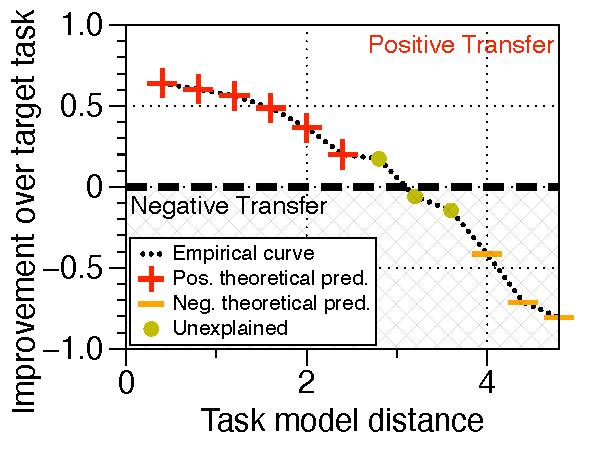
\includegraphics[width=0.98\textwidth]{figures/model_shift_phase_transition.pdf}
		\caption{Task similarity}
		\label{fig_model_shift}
	\end{subfigure}\hfill
	\begin{subfigure}[b]{0.32\textwidth}
		\centering
		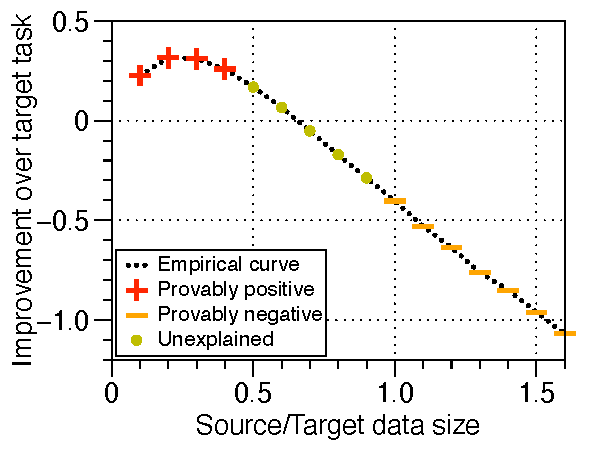
\includegraphics[width=0.98\textwidth]{figures/datapoints_phase_transition.pdf}
		\caption{Sample size}
		\label{fig_size}
	\end{subfigure}\hfill
	\begin{subfigure}[b]{0.32\textwidth}
		\centering
		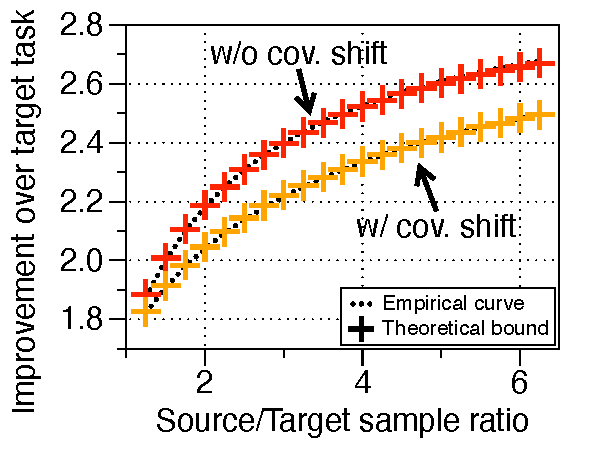
\includegraphics[width=0.98\textwidth]{figures/complementary.pdf}
		\caption{Covariate shift}
		\label{fig_covariate}
	\end{subfigure}
	\caption{%Three takeaways of our theory in Section \ref{sec_insight}.
	We observe a transition from positive to negative transfer as (a) \textit{task model distance} increases and (b) source/target \textit{sample ratio} increases.
	For the special case of having the same task model, we observe in (c) that as source/target \textit{sample ratio} increases, having \textit{covariate shift} worsens the performance of MTL.
	The $y$-axis measures the loss of STL minus MTL.}
	\label{fig_model_shift_phasetrans}
\end{figure}

%\subsection{Sample Ratio}\label{sec_data_size}

\medskip
\noindent{\bf Varying sample ratio.} In classical Rademacher or VC based theory of multi-task learning, the generalization bounds are usually presented for settings where the sample sizes are equal for all tasks \cite{B00,M06,MPR16}.
%More generally, such results are still applicable when all task data are being added simultaneously.
On the other hand, uneven sample sizes between different tasks (or even dominating tasks) have been empirically observed as a cause of negative transfer \cite{YKGLHF20}.
For such settings, we have also observed that adding more labeled data from one task does not always help.
Our theory accurately predicts a curious phenomenon, where increasing the sample size of the source task results in negative transfer!
%On the other hand, we have observed that adding more labeled data does not always improve performance in multi-task learning.

More precisely, in the isotropic model, we consider what happens if we vary the source task sample size. For fixed model distance $pd^2$, the bias term $  pd^2\cdot \frac{\rho_1^2 (\rho_1+\rho_2)}{(\rho_1 + \rho_2 - 1)^3}$ of MTL increases and converges to $pd^2$ as the sample ratio $\rho_1/\rho_2$ increases, and the variance reduction $\frac{\sigma^2}{ \rho_2-1}  -\frac{\sigma^2}{\rho_1+\rho_2-1}$ also increases and converges to $\frac{\sigma^2}{\rho_2-1}$ as $\rho_1/\rho_2$ increases. The tradeoff between these two terms depends on $\rho_1$ in a nonlinear way that is more complicated than the one in the case of varying model distance. But from our results, one can check the following phenomena. If $\frac{\sigma^2}{\rho_2-1} > pd^2$, then the transfer is always positive. On the other hand, if $\frac{\sigma^2}{\rho_2-1} < pd^2$, then there is a transition from the positive transfer to negative transfer as $\rho_1/\rho_2$ increases. 
%Therefore, while the variance of MTL still reduces compared to STL, 
%If the bias increases more than the amount of variance reduced, we will observe negative transfer.
Figure \ref{fig_size} provides a simulation result for such a setting (described in Appendix \ref{app_synthetic}).
%We observe that as $n_1 / n_2$ increases, there is a transition from positive to negative transfer. 
There are several unexplained observations near $y = 0$ caused by the concentration error on the right-hand side of \eqref{cor_MTL_error}.


\iffalse
\begin{proposition}[Source/target sample ratio]\label{prop_data_size}
	In the isotropic model, suppose that $\rho_1 > 40$ and $\rho_2 > 110$ are fixed constants, and $\Psi(\beta_1, \beta_2) > 2/(\rho_2 - 1)$.
	Then we have that
	\begin{itemize}
		\item \textbf{Positive transfer:} If $\frac{n_1}{n_2} = \frac{\rho_1}{\rho_2} < \frac{1}{\nu} \cdot \frac{1 - 2\rho_2^{-1}}{\Psi(\beta_1, \beta_2) (\rho_2 - 1) - \nu^{-1}}$, then w.h.p. $$\te(\hat{\beta}_2^{\MTL}) < \te(\hat{\beta}_2^{\STL}).$$
		\item \textbf{Negative transfer:} If $\frac{n_1}{n_2} = \frac{\rho_1}{\rho_2} > {\nu} \cdot \frac{1 - 2\rho_2^{-1}}{\Psi(\beta_1, \beta_2) (\rho_2 - 3/2) - \nu}$, then w.h.p. $$\te(\hat{\beta}_2^{\MTL}) > \te(\hat{\beta}_2^{\STL}).$$
	\end{itemize}
\end{proposition}
Proposition \ref{prop_data_size} describes the bias-variance tradeoff in terms of the sample ratio $\rho_1 / \rho_2$.


We apply the result to the setting of Figure \ref{fig_size} (described in Appendix \ref{app_synthetic}).
There are several unexplained observations near $y = 0$ caused by $\nu$.
The proof of Proposition \ref{prop_data_size} can be found in Appendix \ref{app_proof_32}.
\fi

\subsection{Covariate Shift} \label{sec_covshift}
So far we have considered the isotropic model where $\Sigma_1 = \Sigma_2$.
This setting is relevant for settings where different tasks share the same input features such as multi-class image classification.
In general, the covariance matrices of the two tasks may be different such as in text classification.
In this part, we consider what happens when $\Sigma_1 \neq \Sigma_2$.
We show that when $n_1 / n_2$ is large, MTL with covariate shift can be suboptimal compared to MTL without covariate shift.

%\noindent\textit{Example.}

\begin{example}
	We measure covariate shift by the transfer matrix $M = \Sigma_1^{1/2} \Sigma_2^{-1/2}$. %similar to Theorem \ref{thm_main_informal}.
	We assume that the two tasks have the same ground truth model parameters, that is, $\beta_1 = \beta_2$.
	We compare two cases: (i) when $M = \id_{p\times p}$; (ii) when $M$ has $p/2$ singular values that are equal to $\lambda$ and $p/2$ singular values that are equal to $1 / \lambda$.
	Hence, $\lambda$ measures the severity of the covariate shift.
	Figure \ref{fig_covariate} shows a simulation of this setting by varying $\lambda$.
	We observe that as source/target sample ratio increases, the performance gap between the two cases increases.
	\end{example}

%By applying Lemma \ref{lem_cov_shift_informal}, we find that when $n_1 / n_2$ is large, having no covariate shift is the optimal choice provided that the determinant of $M^{\top}M$ is bounded.
We compare different choices of $M$ that belong to the following bounded set.
Let $\lambda_i$ be the $i$-th singular value of $M$.
Let $\mu_{\min} < \mu < \mu_{\max}$ be fixed values that do not grow with $p$.
{\begin{align*}
		\cS_{\mu}\define\bigset{M \left| \prod_{i=1}^p \lambda_i \le \mu^p, \mu_{\min} \le \lambda_i\le \mu_{\max}, \text{ for all } 1\le i\le p\right.}.
\end{align*}}
%	We assume that $\beta_1$ and $\beta_2$ are generated following the isotropic model with $d = 0$.
\begin{proposition}[Covariate shift]\label{prop_covariate}
	For the setting of the example above, assume that $\beta_1 = \beta_2$, $\rho_1$ and $\rho_2$ are both greater than one.
	Let $g(M)$ denote the prediction loss of $\hat{\beta}_t^{\MTL}$ when $M = \Sigma_1^{1/2}\Sigma_2^{-1/2} \in\cS_{\mu}$.
	We have that
		\[ g(\mu\id) \le \bigbrace{1+ \bigo{{\rho_2}/{\rho_1}  }} \min_{M\in\cS_{\mu}} g(M). \]
\end{proposition}


\iffalse

 \begin{claim}\label{claim_covar_shift}
		In the setting of Proposition \ref{prop_covariate}, for any $M\in \cal S_\mu$ we have that
		\[ g(M)=(1+\OO(p^{-\e}))\cdot \sigma^2  \bigtr{\Sigma_2(X_1^{\top}X_1  + X_2^{\top}X_2)^{-1} }  \quad \text{w.h.p.} \]
	\end{claim}

%Finally, in this subsection we prove Proposition \ref{prop_covariate}, which shows that $\te(\hat{\beta}_2^{\MTL})$ is minimized approximately when $M$ is a scalar matrix, provided that there is enough source data.

\begin{proof}[Proof of Proposition \ref{prop_covariate}]
 

 
 Denote the minimizer of $g$ by 
$$M_0:=\argmin_{M\in \cal S_{\mu}}g(M).$$ 
We now calculate $g(M_0)$. 


Now using Lemma \ref{lem_cov_shift}, we obtain that with high probability,
\begin{align}\label{gvar_extra}
g(M_0)= \frac{\sigma^2}{\rho_1+\rho_2}\cdot \frac1p\tr\left( \frac{1}{a_1(M_0)\cdot M_0^\top M_0 + a_2(M_0)}\right) \cdot \left(1 +\OO(p^{-\e})\right).
\end{align}
From equation \eqref{eq_a12extra}, it is easy to obtain the following estimates on $ a_1(M)$ and $a_2(M)$ for any $M\in \cal S_\mu$:
\be\label{est_a12extra}
\frac{\rho_1-1}{\rho_1+\rho_2} < a_1(M)<  \frac{\rho_1+\rho_2-1}{\rho_1+\rho_2},\quad a_2(M) < \frac{\rho_2}{\rho_1+\rho_2}.
\ee
Inserting \eqref{est_a12extra} into \eqref{gvar_extra} and using $ M_0^\top M_0\succeq \mu_{\min}^2$, we obtain that with high probability,
\begin{align}\label{approximateteM}
\left(1+\frac{\rho_2}{(\rho_1-1)\mu_{\min}^2}\right)^{-1}h(M_0) \cdot \left(1 - \OO(p^{-\e})\right) \le g(M_0) \le h(M_0) \cdot \left(1 +\OO(p^{-\e})\right),
\end{align}
where
$$h(M_0):=\frac{\sigma^2}{(\rho_1+\rho_2)a_1(M_0)}\cdot \frac1p\tr\left( \frac{1}{M_0^\top M_0}\right) .$$
%With these two bounds, we can easily conclude \eqref{approxteM}. 
%
%We have that the test error satisfies
%\be\label{approxteM}  te(M)\left(1 -  \frac{n_2}{n_1-p} \frac{1}{\lambda_p^2 + \frac{n_2}{n_1-p}}\right)  \le  \frac{\sigma^2}{n_1+n_2}\tr\left( \frac{1}{a_1M^\top M + a_2}\right) \le te(M),\ee
%where $\lambda_p$ is the smallest singular value of $p$ and
%$$te(M):= \frac{\sigma^2}{a_1(n_1+n_2)}\tr\left( \frac{1}{M^\top M}\right) .$$
%Moreover, for all $M$ satisfying \eqref{GMcons}, the minimum of $te(M)$ is attained when $M= a\id$.
By AM-GM inequality, we observe that 
$$\tr\left( \frac{1}{M^\top M}\right) = \sum_{i=1}^p\frac{1}{\lambda_i^2}$$
is minimized when $\lambda_1 = \cdots\lambda_p=\mu$ under the restriction $\prod_{i=1}^p\lambda_i\le \mu^p$. Hence we get that 
\be\label{AMGM} h(M_0) \le \frac{\sigma^2}{\mu^2 (\rho_1+\rho_2)a_1(M_0)}.\ee
On the other hand, when $M=\mu \id$, applying Lemma \ref{lem_cov_shift} we obtain that with high probability,
\begin{align}\label{gvar_extra2}
\begin{split}
g(\mu \id)&= \frac{\sigma^2}{\rho_1+\rho_2}\cdot \frac1p\tr\left( \frac{1}{\mu^2 a_1 (\mu\id) + a_2(\mu\id)}\right) \cdot \left(1 +\OO(p^{-\e})\right)\\
&\le \frac{\sigma^2}{\mu^2(\rho_1+\rho_2)a_1 (\mu\id)}.
\end{split}
\end{align}
Combining \eqref{est_a12extra}, \eqref{approximateteM}, \eqref{AMGM} and \eqref{gvar_extra2}, we conclude the proof.
%, we conclude that the sum $\sum_{i=1}^p\lambda_i^{-1}$ is smallest when $\lambda_1=\cdots=\lambda_p = a$.
\end{proof}
\fi

Proposition \ref{prop_covariate} shows that when the sample ratio is large, having no covariate shift gives the optimal performance for multi-task learning.
The proof of Proposition \ref{prop_covariate} can be found in Appendix \ref{app_proof_33}.
%Proposition \ref{prop_covariate} implies that when $\rho_1\gg \rho_2$, having no covariate shift is the optimal choice for choosing the source task.
%This provides evidence that covariate shift is unfavorable when there are many source task datapoints,

%\todo{} To complement the result, we show an example when the statement is not true if $n_1 \le n_2$.

%We ask: is it better to have $M$ as being close to identity, or should $M$ involve varying levels of singular values?
%Understanding this question has implications for applying normalization methods in multi-task learning \cite{LV19,CBLR18,YKGLHF20}.
%We show that if $n_1$ is much larger than $n_2$, then the optimal $M$ matrix should be proportional to identity, under certain assumptions on its range of singular values (to be formulated in Proposition \ref{prop_covariate}).
%On the other hand, if $n_1$ is comparable or even smaller than $n_2$, we show an example where having ``complementary'' covariance matrices is better performing than having the same covariance matrices.



\subsection{Sample Efficiency}

observed in Taskonomy \cite{ZSSGM18}.




\section{Empirical results}


%\subsection{Comparison between the averaging and HPS estimators}
\paragraph{Regression tasks.}

\paragraph{Text classification.}
Our results and simulations are all in the high-dimensional linear regression setting.
How well do they extend to other scenarios?
In this section, we conduct further studies on six text classification datasets.
Our datasets include a movie review sentiment dataset (MR) \cite{pang2005seeing}, a sentence subjectivity dataset (SUBJ) \cite{pang2004sentimental}, a customer reviews dataset (CR) \cite{hu2004mining}, a question type dataset (TREC) \cite{li2002learning}, an opinion polarity dataset (MPQA) \cite{wiebe2005annotating}, and the Stanford sentiment treebank (SST) dataset \cite{socher2013recursive}.
%The question is to predict positive or negative sentiment expressed in the text.
Our model consists of a word embedding layer with GloVe embeddings \cite{pennington2014glove} followed by a long-short term memory (LSTM) or a multi-layer perception (MLP) layer \cite{lei2018simple}.\footnote{For MLP, we apply an average pooling layer over word embeddings. For LSTM, we add a shared feature representation layer on top of word embeddings.}


\subsection{Covariate alignment}


\paragraph{Covariate shift}
Recall from Example \ref{ex_covshift} that having covariate shifts worsens the variance (hence the loss) of hard parameter sharing when the sample ratio increases.
This highlights the need for correcting covariate shifts when the sample size ratio rises.
To this end, we study a covariance alignment procedure proposed in \cite{WZR20}, designed to correct covariate shifts.
The idea is to add an alignment module between the input and the shared module $B$.
This module is then trained together with $B$ and the output layers. We refer to \cite{WZR20} for more details about the procedure and the implementation.
%We validate our insight on this procedure in the experiments.
%We implement the covariance alignment procedure following \cite{WZR20}.

We conduct multi-task training on all $15$ task pairs from the six datasets.
In Figure \ref{fig_ab_cov}, we measure the performance gains from performing covariance alignment vs. HPS.
To get a robust comparison, we average the improvements over the 15 task pairs.
The result shows that as the sample size ratio increases, performing covariance alignment provides more significant gains over HPS.
We fix task two's sample size at $1,000$, and increase task one's sample size from $1,000$ to $3,000$.



%One estimator that is sometimes employed in the literature is simply an average of the OLS estimators for two tasks \cite{bastani2020predicting}
%\be\label{eq_est_ave}\hat \beta^{\AV}(\lambda)=\lambda \cdot \hat \beta_1^{\STL}+ (1-\lambda)\cdot \hat \beta_2^{\STL},\ee
%where $\lambda\in [0,1]$ is an averaging parameter subject to choice in practice, and we recall that the OLS estimators are given by
%$$\hat \beta_i^{\STL}= [(X^{(i)})^\top X^{(i)}]^{-1}(X^{(i)})^\top Y^{(i)},\quad i=1,2.$$
%The estimator in \eqref{eq_est_ave} is conventionally called an \emph{averaging estimator}.
%In particular, when $\lambda=0$ and $1$, we get the OLS estimators for tasks 2 and 1, respectively.

%\section{Experimental results}

\subsection{Progressive training}%\label{sec_text}


%multi-layer perceptron (MLP), LSTM, CNN on all tasks
%We use this task to verify our theoretical results on model capacity and task covariance in real world.
%{\it ChestX-ray14.} This dataset contains 112,120 frontal-view X-ray images \cite{chexnet17}.
%There are 14 diseases (tasks) for every image that we would like to predict.
%We use densenet121 as the shared module \cite{huang2017densely}.
%We treat each label as one task a binary classification problem and formulate it as a 14-task multi-task learning problem.
%This dataset is curated where the labels
%We use the CheXNet model from~\cite{chexnet}, which is a 121-layer convolutional neural network on all tasks.
%For the text classification experiment, we encode each word using the GLoVe word embeddings.%
%\footnote{http://nlp.stanford.edu/data/wordvecs/glove.6B.zip}
%We evaluate three model choices.
%\textit{Predicting transfer effect via STL results.}
%We show that the single-task based metric proposed in Section \ref{sec_similarity} can predict positive or negative transfer in MTL.
%A common challenge in the study of MTL is that the results can be hard to understand.
%It is difficult to predict when MTL performs well without running extensive trials.
%Our insight is that we can use STL results to help understand MTL results.
%Table \ref{tab:mtl_better_than_stl} shows the result on both the sentiment analysis and the ChestX-ray14 tasks.
%We find that using a threshold of $\tau = 0.1$, the STL results correctly predict positive or negative transfer with $75.6\%$ precision and $38.8\%$ recall among $30$ times $5$ (random seeds) task pairs!
%We observe similar results for $91$ task pairs from the ChestX-ray14 dataset.
%The results show that STL results are indicative of MTL results.

\paragraph{Sample size ratio.}
First, we we show that our observation in Figure \ref{fig_size} also occurs in the text classification tasks.
In Figure \ref{fig_ab_data}, we observe that for multiple example task pairs, increasing task one's sample size improves task two's prediction accuracy initially, but hurts eventually.
On the $y$-axis, we plot task two's test accuracy using HPS, subtracted by its STL test accuracy.
%validate that as we increase the sample ratio while keeping task two's sample size fixed, task two's prediction accuracy does not always increase.
We fix task two's sample size at $1000$ and increase task one's sample size from $100$ to $3000$.

These examples and the one in Figure \ref{fig_size} suggest a natural progressive training schedule, where we add samples progressively until performance drops.
Concretely, here is one implementation of this idea.
%In particular, Figure \ref{fig_size} (and our analysis) shows that $L(\hat{\beta}_t^{\MTL})$ behaves as a quadratic function over $\rho_1$.
%More generally, depending on how large $\Psi(\beta_1, \beta_2)$ is, $L(\hat{\beta}_t^{\MTL})$ may also be monotonically increasing or decreasing.
%Based on this observation, we propose a progressive training schedule to improve the compuational efficiency of hard parameter sharing.
\begin{itemize}
	\item We divide the training data into $S$ batches.
	We divide the training procedure into $S$ stages. During every stage, we progressively add one more data batch.
	\item During every stage, we train for $T$ epochs using only the $S$ batches. If the validation accuracy drops compared to the previous round's result or reach a desired threshold $\tau$, we terminate.
%	Algorithm \ref{alg_inc_train} in Appendix \ref{app_experiments} describes the procedure in detail.
\end{itemize}
If we apply this procedure to the settings of Figure \ref{fig_ab_data} and \ref{fig_size}, it will terminate once reaching the optimal sample ratio.
%See Algorithm \ref{alg_inc_train} for a complete description for two tasks.
The advantage of this procedure is that it reduces the computational cost compared to standard round-robin training schedules.
For example, if the procedure terminates at 30\% of all batches, then SGD only passes over 30\% of its data, whereas standard round-robin training passes over 100\% of task one's data.

\begin{algorithm}[!t]
	\caption{An incremental training schedule for efficient multi-task learning with two tasks}
	\label{alg_inc_train}
	\begin{algorithmic}[1]
		\Input Two tasks $(X_1, Y_1)$ and $(X_2, Y_2)$.
		\Param A shared module $B$, output layers $W_1, W_2$ as in the hard parameter sharing architecture.
		\Req \# batches $S$, epochs $T$, task $2$'s validation accuracy $\hat{g}(B; W_2)$, a threshold $\tau\in(0,1)$.
		\Output The trained modules $B, W_2$ optimized for task $2$.
		\State Divide $(X_1, Y_1)$ randomly into $S$ batches: $(x^{(1)}, y^{(1)}), \dots, (x^{(S)}, y^{(S)})$.
		\For{$i = 1,\dots, S$}
		\For{$j = 1,\dots, T$}
		\State Update $B, W_1, W_2$ using the training data $\set{x^{(k)}, x^{(k)}}_{k=1}^i$ and  $(X_2, Y_2)$.
		\EndFor
		\State Let $a_i = \hat{g}(B; W_2)$ be the validation accuracy.
		\If{$a_i < a_{i-1}$ or $a_i > \tau$}
		\State \textbf{break}
		\EndIf
		\EndFor
	\end{algorithmic}
\end{algorithm}

%We fill in the details of the experimental procedure used for the results in Figure \ref{fig_ablation}.
%\squishlist
%	\item Task similarity: We select a similar and a dissimilar source task compared to the target task using domain knowledge.
%First pair: the customer review dataset (CR) , which predicts whether a review is positive or negative, is more similar to SST (sentiment treebank) than MPQA (question type).
%Second pair: SST is more similar to MR since they both concern about positive or negative opinions expressed the text.
%TREC is less similar to MR because the task is about question types.
%Third pair: MPQA (opinion polarity) is more similar to TREC (question type)
We evaluate the progressive training procedure on the six text classification datasets.
First, we conduct multi-task training over all $15$ two-task pairs from the six datasets.
We focus on task two's test accuracy and set $\tau$ as task two's test accuracy obtained via the standard round-robin training schedule.
We include all of task two's data and progressively add task one's data using the procedure described above.
Since the prediction accuracy has been controlled the same, we compare the computational cost.
We find that when averaged over all $15$ two-task pairs, this procedure requires only $45\%$ of the computational cost to reach the desired accuracy $\tau$ for task two.
%Our insight is that since adding more samples from the source task does not always help, we can improve efficiency by adding source samples \textit{progressively} during training.
%\textbf{Improving transfer learning training efficiency.}
%We show that Algorithm \ref{alg_inc_train} also applies to transfer learning settings.
%Compared to fine-tuning the source model on the target task, we show that our proposed method reduces the computional cost by \alert{$xx\%$}, without sacrificing accuracy.
Second, we conduct multi-task training on all six datasets jointly.
We extend our procedure to all six datasets. We include the data from all tasks except SST. For SST, we progressively add data similar to the above procedure.
We set $\tau$ to be the average test accuracy of all six tasks obtained using standard round-robin training.
We find that adding samples progressively from SST requires less than $35\%$ of the computational cost to reach the same average test accuracy $\tau$.

\subsection{Width selection}
%As a further validation, excluding TREC, we observe similar comparative results.
%The data efficiency ratio of using MLP is $100\%$ because the average performance of MTL is worse than the average of STL.
%We further show that applying incremental training helps reduce the data efficiency ratio to \alert{$xx\%$}.
%If TREC is not included, we see that only $25\%$ of the labeled data is needed.



%	\begin{subfigure}[b]{0.33\textwidth}
%		\centering
%		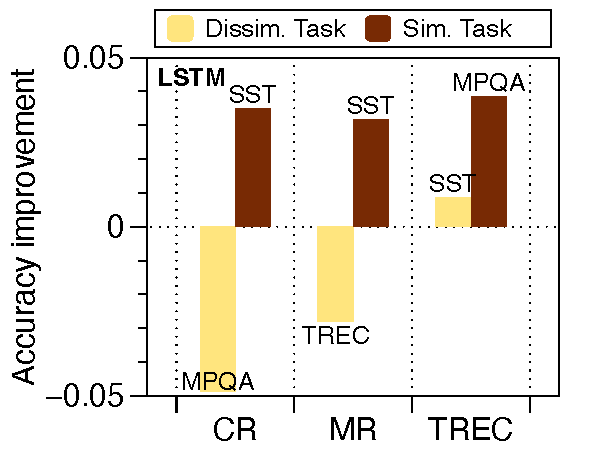
\includegraphics[width=0.975\textwidth]{figures/task_sim_norm_lstm.pdf}
%		\caption{Task similarity}
%		\label{fig_ab_sim}
%	\end{subfigure}%
%	\caption{Validating the three results of Section \ref{sec_insight} on sentiment analysis tasks. (a) Adding a semantically similar source task in MTL performs better than adding a dissimilar task.
%	(b) As source/target sample ratio increases, we observe a transition from positive to negative transfer.
%	(c)
%	Note: (S) denotes the source task and (T) denotes the target task.}


%\begin{minipage}[t]{.58\textwidth}
%	\vspace{-0.1in}
%	\centering
%  \begin{tabular}{c c c c c}
%	\toprule
%		\multirow{2}{*}{{\bf Threshold}}  & \multicolumn{2}{c}{{\bf Sentiment
%		analysis}} & \multicolumn{2}{c}{{\bf ChestX-ray14}} \\
%		& Precision &  Recall & Precision &  Recall \\
%		\cmidrule(lr){1-1} \cmidrule(lr){2-3} \cmidrule(lr){4-5}
%		0.0 & 0.596 & 1.000 & 0.593 & 1.000 \\
%		0.1 & \textbf{0.756} & \textbf{0.388} & \textbf{0.738} & \textbf{0.462} \\
%		0.2 & 0.919 & 0.065 & 0.875 & 0.044 \\
		% 0.3 & 1.000 & 0.004 &     - &     - \\
%	\bottomrule
%	\end{tabular}
%	\vspace{0.1in}
%	\captionof{table}{Single-task learning results can help predict postive or negative transfer in multi-task learning.}
%	\label{tab:mtl_better_than_stl}
%\end{minipage}%
%\quad



%\begin{figure}[!t]
%	\centering
%	\begin{subfigure}[b]{0.5\textwidth}
%		\centering
%		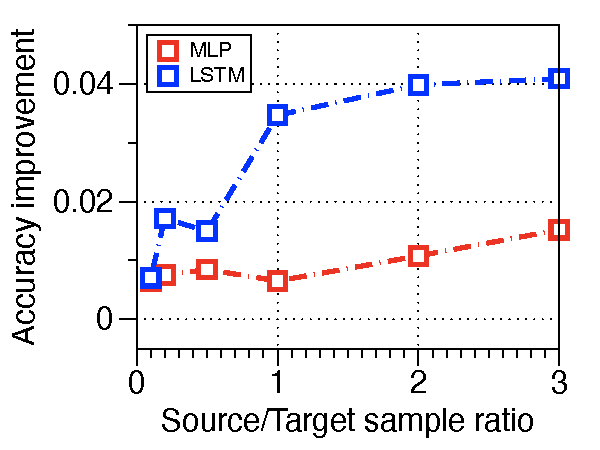
\includegraphics[width=0.5\textwidth]{figures/ratio_alignment_norm_diff_all.pdf}
%		\caption{Averaged over all 16 task pairs}
%		\label{fig_ab_cov}
%	\end{subfigure}\hfill
%	\begin{subfigure}[b]{0.5\textwidth}
%		\centering
%		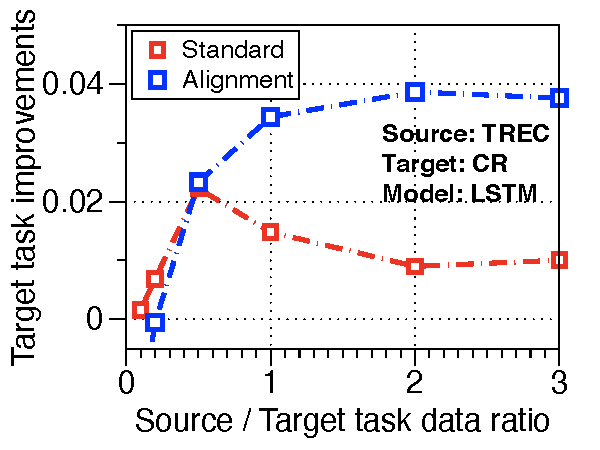
\includegraphics[width=0.5\textwidth]{figures/ratio_alignment_norm_trec_cr_lstm.pdf}
%		\caption{An example task pair}
%		\label{fig_cov_a}
%	\end{subfigure}
%	\caption{ (TREC and CR)}
%\end{figure}

%\textbf{Further results of the covariance alignment procedure.}
%Our results in Figure \ref{fig_ab_cov} are averaged over all the task pairs.
%In Figure \ref{fig_covariate_app}, we show two task pairs as examples.
%In Figure \ref{fig_cov_a}, we observe that for the particular task pair, covariance alignment provides more significant gains when the sample ratio is large.
%In Figure \ref{fig_cov_b}, we observe that covariance alignment does not always improve over the baseline multi-task learning model.
%One explanation is that MR and SST are similar tasks, hence adding the alignment module is unnecessary.
%An interesting question is to understand when adding the alignment module benefits the multi-task learning model.
%We leave this question for future work.
%Note: For text classification tasks, the source task training data size ranges from 500 to 1,500 and target task training data size is 1000; For ChestX-ray14,

%\begin{figure}[!h]
%	\centering
%	\begin{subfigure}[b]{0.48\textwidth}
%		\centering
%		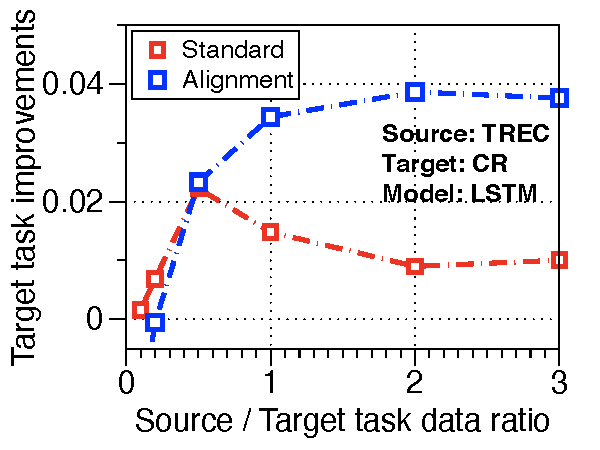
\includegraphics[width=0.7\textwidth]{figures/ratio_alignment_norm_trec_cr_lstm.pdf}
%		\caption{Task pair TREC and CR}
%		\label{fig_cov_a}
%	\end{subfigure}\hfill
%		\begin{subfigure}[b]{0.48\textwidth}
%		\centering
%		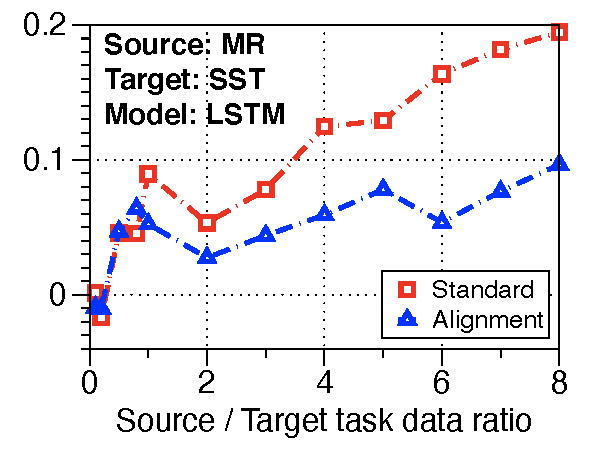
\includegraphics[width=0.7\textwidth]{figures/ratio_alignment_mr_sst_lstm.pdf}
%		\caption{Task pair MR and SST}
%			\label{fig_cov_b}
%	\end{subfigure}
%	\caption{(a) For the task pair TREC and CR, adding the covariance alignment procedure provides more improvement when the source/target sample ratio is large.
%	(b) For the task pair MR and SST, adding the covariance alignment procedure hurts performance.
%	One explanation is that MR and SST are similar tasks, hence adding the alignment module is unnecessary.}
%	\label{fig_covariate_app}
%\end{figure}


\begin{figure}%[!t]
	\begin{subfigure}[t]{0.5\textwidth}
		\centering
		\vspace{0pt}
		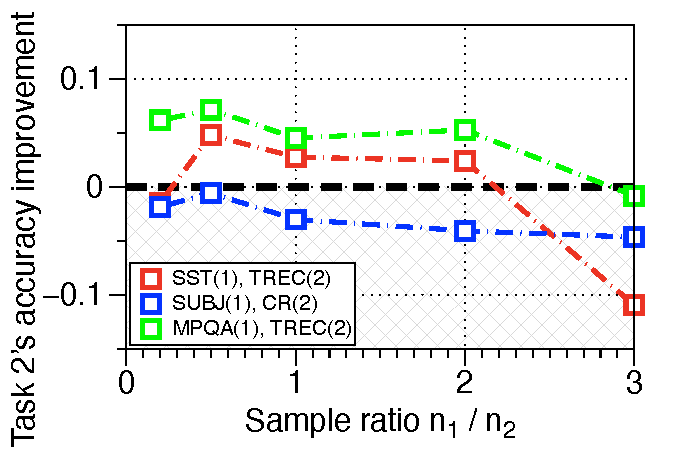
\includegraphics[width=0.8\textwidth]{figures/fig3a.pdf}
		\caption{HPS vs. STL}
		\label{fig_ab_data}
	\end{subfigure}\hfill
	\begin{subfigure}[t]{0.5\textwidth}
		\centering
		\vspace{0pt}
		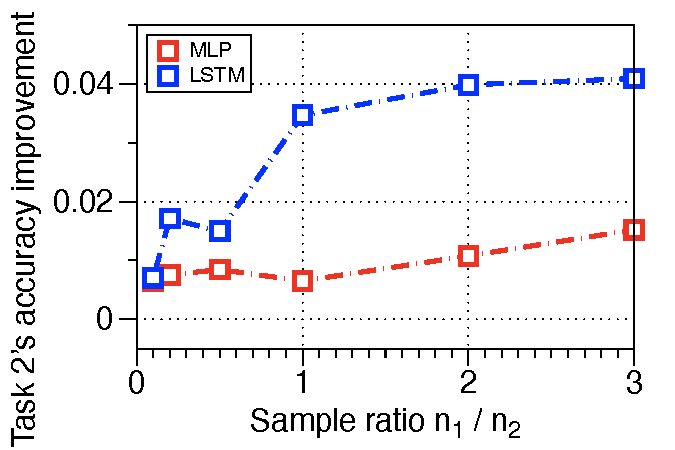
\includegraphics[width=0.8\textwidth]{figures/fig3b.pdf}
		\caption{HPS vs. covariance alignment}
		\label{fig_ab_cov}
	\end{subfigure}
	\caption{Comparing hard parameter sharing (HPS) to single-task learning (STL) and a covariance alignment approach proposed by \cite{WZR20}:
	In Figure \ref{fig_ab_data}, we observe that for multiple task pairs, increasing task one's sample size improves task two's prediction accuracy initially, but hurts eventually -- a phenomenon similar  to Figure \ref{fig_size}.
	In Figure \ref{fig_ab_cov}, we observe that as task one's sample size increases, covariance alignment improves more over HPS.}
	\label{fig_text}
%	\begin{minipage}[t]{0.4\textwidth}
%		\centering
%		\vspace{0pt}
%		\begin{tabular}{c c c}
%		\toprule
		% \multirow{2}{*}{{\bf Models}} & \multicolumn{2}{c}{\begin{minipage}{1.2in}\begin{center}
		% Sentiment\\ analysis\end{center}\end{minipage}} \\
%		\multirow{2}{*}{{\bf Models}} & \multicolumn{2}{c}{\bf Sentiment analysis} \\
		% \cmidrule(lr){2-3}
%		& all tasks & w/o TREC \\
%		\midrule
%		{\bf MLP}  & 31\% & 29\% \\
%		{\bf LSTM} & 35\% & 34\% \\
%		{\bf CNN}  & 30\% & 28\% \\
%		\bottomrule
%		\end{tabular}
%		\captionof{table}{Finding the best sample ratio via a progressive training schedule.}
%		\label{tab:taskonomy}
%	\end{minipage}
\end{figure}

%\begin{algorithm}[!t]
%	\caption{A progressive training schedule given two tasks}
%	\label{alg_inc_train}
%	\begin{algorithmic}[1]
%		\Input Two tasks $(X^{(1)}, Y^{(1)})$ and $(X^{(2)}, Y^{(2)})$.
%		\Param A shared module $B$, output layers $A_1, A_2$ as in the hard parameter sharing architecture.
%		\Req \# batches $S$, epochs $T$, task $2$'s validation accuracy $\hat{g}(B; W_2)$, a threshold $\tau\in(0,1)$.
%		\Output The trained modules $B, A_2$ optimized for task $2$.
%		\State Divide $(X^{(1)}, Y^{(1)})$ randomly into $S$ batches: $(x^{(1)}, y^{(1)}), \dots, (x^{(S)}, y^{(S)})$.
%		\For{$i = 1,\dots, S$}
%			\For{$j = 1,\dots, T$}
%				\State Update $B, A_1, A_2$ using the training data $\set{x^{(k)}, x^{(k)}}_{k=1}^i$ and  $(X^{(2)}, Y^{(2)})$.
%			\EndFor
%			\State Let $a_i = \hat{g}(B; A_2)$ be the validation accuracy.
%			\If{$a_i < a_{i-1}$ or $a_i > \tau$}
%				\State \textbf{break}
%			\EndIf
%		\EndFor
%	\end{algorithmic}
%\end{algorithm}

\section{Extension to multiple data sources}\label{sec_same}

Our setup and the results in Section \ref{sec_main} are both for transferring from one data source.
This section extends our setup to transfer learning from multiple data sources.
We focus on a natural setting where all the tasks have the same covariates but different labels.

\paragraph{Data model.} Suppose we have $t$ datasets whose sample sizes are all equal to $n$ and whose feature covariates are all equal to $X \in \real^{n \times p}$. The label vector of the $i$-th task follows a linear model
\begin{align}\label{eq_mtl_data}
    Y^{(i)} = X \beta^{(i)} + \varepsilon^{(i)}, \text{ for } i=1, 2,\cdots, t.
\end{align}
Similar to Section \ref{sec_main}, we use the first $(t-1)$ datasets as sources to predict the $t$-th task.
However, there is a \text{model shift} between the data sources and the task we would like to predict.
We make several standard assumptions on $X$ and each of $\varepsilon^{(i)}$.
First, $X = Z\Sigma^{1/2}$ is a random matrix satisfying Assumption \ref{assm_big1} (same as $X^{(2)}$).
In particular, the sample size $n$ is greater than the dimension $p$.
Second, every $\varepsilon^{(i)} \in \real^{n}$ is a random vector with i.i.d entries of mean zero, variance $\sigma^2$, and bounded moments up to any order (cf. equation \eqref{eq_highmoments}).
Finally, $\beta^{(i)} \in \real^{p}$ is a fixed vector independent from any other $\beta^{(j)}$ for $j \neq i$, the matrix $X$, and $\varepsilon^{(j)}$ for any $j$.

\paragraph{Estimator.} We combine multiple data sources by extending the two-layer linear neural network from equation \eqref{eq_hps} as follows:
\begin{align}
	f(A, B) = \sum_{j=1}^t \bignorm{X B A_j - Y^{(j)}}^2, \label{eq_mtl_same_cov}
\end{align}
where $A = [A_1, A_2, \dots, A_t] \in \real^{r \times t}$ denotes the output layer and $B \in \real^{p \times r}$ denotes the (shared) feature layer.
We set the width of the feature layer $r$ less than the number of tasks $t$.
Otherwise, when $r \ge t$, the global minimum of $f(A, B)$ reduces to single-task learning, similar to Proposition \ref{prop_large_r} (details omitted).

Let $(\hat A, \hat B)$ denote a global minimizer of $f(A, B)$.
We define the HPS estimator for task $t$ as $\hat \beta_t^{\MTL} := \hat B \hat A_i$, where $\hat A_i$ denotes the $i$-th column of $\hat A$.
We evaluate the performance of $\hat{\beta}_t^{\MTL}$ according to its excess risk:
\be\label{ith_loss}
    L_t(\hat{\beta}_t^{\MTL}) = \bignorm{\Sigma^{1/2} \left(\hat{\beta}^{\MTL}_t - \beta^{(t)}\right)}^2.
\ee

\paragraph{Result.} We show that in the multi-task setting, hard parameter sharing finds the ``best'' rank-$r$ approximation to all tasks.
To formally describe our result, we introduce several notations.
Let $B^\star \define [{\beta}^{(1)},{\beta}^{(2)},\dots,{\beta}^{(t)}] \in \real^{p\times t}$ be the concatenated model vectors of all tasks.
Let $A^{\star} {A^{\star}}^{\top}$ be the best rank-$r$ approximation of ${B^{\star}}^\top\Sigma B^{\star}$ in the following sense:
\begin{align}\label{eq_A_star}
	A^{\star} \define \argmin_{U\in\real^{t\times r} : U^{\top} U = \id_{r\times r}} \inner{U U^{\top}} {{B^{\star}}^{\top} \Sigma B^{\star}},
\end{align}
where $\langle \cdot ,\cdot \rangle $ denotes the Frobenius inner product between two matrices.
Let $a_i^{\star}\in\real^r$ be the $i$-th column vector of $A^{\star}{A^{\star}}^{\top}$.
We characterize the excess risk $L_t(\hat{\beta}_t^{\MTL})$ precisely in the following result.

\begin{theorem}[Excess risk of HPS for multiple tasks under model shift]\label{thm_many_tasks}
Suppose the multi-task setting according to equation \eqref{eq_mtl_data} holds.
Let $r$ be any positive integer less than $t$.
Suppose the $r$-th largest eigenvalue of ${B^\star}^\top \Sigma B^\star$ is strictly larger than its $(r+1)$-th largest eigenvalue. 
Let $c>0$ be an arbitrary (small) constant.
The following estimates for $L_t(\hat{\beta}_t^{\MTL})$ holds with high probability:
\begin{align}
	\bigabs{L_t(\hat{\beta}_t^{\MTL}) - L_t(B^{\star}a_t^{\star}) -\frac{p\sigma^2}{n-p}  \norm{a_t^{\star}}^2} 
	\le  \sqrt{\bignorm{{B^\star}^\top\Sigma B^\star}_{\op} \cdot n^{-\frac 1 2+ \frac 2{\varphi} + c}  + \sigma^2 n^{-\frac 1 2 + c}} \cdot \frac{\bignorm{{B^\star}^\top\Sigma B^\star}_{\op}+  \sigma^2}{\lambda_r - \lambda_{r+1}}. \label{Li_multi1}
\end{align}
	%where $\lambda_r({B^\star}^\top\Sigma B^\star)$ and $\lambda_{r+1}({B^\star}^\top\Sigma B^\star)$ are respectively be the $r$-th and $(r+1)$-th largest eigenvalue of ${B^\star}^\top\Sigma B^\star$.
%	where $C_1: = \frac{\bignormFro{\Sigma^{1/2} B^{\star}}^2 + \sigma^2 t}{\lambda_r ({B^\star}^\top \Sigma B^\star)- \lambda_{r+1}({B^\star}^\top \Sigma B^\star)}$. %and $C_2 :=  C_1\cdot \norm{\Sigma^{1/2} B^{\star}}$.
%Finally, we have a better bound for the averaged prediction loss:  with high probability,
%\begin{align}
%&\left|\frac{1}{t}\sum_{i=1}^t L_i(\hat{\beta}_i^{\MTL}) - \frac1t\bignorm{\Sigma^{1/2} B^{\star} (A^\star {A^\star}^{\top} - \id_{t\times t})}_F^2 - \frac{p \sigma^2}{n-p}\cdot \frac{r}{t}  \right| \nonumber \\
% &\le n^{-1/2+2/\varphi+c}  \norm{{B^\star}^\top\Sigma B^\star}+ n^{-1/2+c}   \sigma^2 .\label{Li_multi2}
%\end{align}
\end{theorem}


Recall that $\varphi > 4$ according to Assumption \ref{assm_big1}, thus, $\frac {2}{\varphi} \le \frac 1 2$ and $n^{-\frac 1 2 + \frac 2 {\varphi} + c}$ vanishes to zero for a small enough constant $c$.
Therefore, equation \eqref{Li_multi1} precisely characterizes the excess risk of the HPS estimator.
As a remark, the same result applies to any other tasks although we have focused on predicting task $t$.
Theorem \ref{thm_many_tasks} significantly extends the two-task model shift setting of Theorem \ref{cor_MTL_loss}.
The term $L_t(B^{\star} a_t^{\star})$ captures the bias of the HPS estimator and $\frac{p \sigma^2}{n - p} \bignorm{a_t^{\star}}^2$ captures the estimator's variance.
%The bound \eqref{minimizer_beta} verifies our intuition that hard parameter sharing approximates the matrix ${B^{\star}}^\top\Sigma B^{\star}$ through a best rank-$r$ subspace. The estimate \eqref{Li_multi1}
% gives the exact asymptotic limit of $L_i(\hat{\beta}_i^{\MTL}(\hat a))$, which shows that the prediction loss of $\hat{\beta}_i^{\MTL}$ decomposes into a bias term $L_i(B^{\star} a_i^{\star})$ that measures the prediction loss of $B^{\star} a_i^{\star}$, plus a variance term that scales with $\norm{a_i^{\star}}^2$. Since $\norm{a_i^{\star}}^2\le 1$, compared with the single-task predication loss \eqref{L_STL_simple01}, the variance term always decreases for the multi-task HPS estimator. On the other hand, the bias term always increases (because the bias in single-task linear regression is zero). Hence as in the transfer learning setting, whether the HPS estimator is better than the OLS estimator depends on an intricate  {bias-variance tradeoff}.
%{\cor One direct implication of our result is that compared to STL, the variance always decreases, since STL's variance is equal to $\sigma^2 \tr[\Sigma (X^{\top} X)^{-1}]$.
%On the other hand, the bias always increases.}
%We can observe a similar {bias-variance tradeoff} for the averaged predication loss in \eqref{Li_multi2} using the fact that $r<t$. Note that the estimate \eqref{Li_multi2} can be applied even when the best rank-$r$ subspace approximation of ${B^{\star}}^\top\Sigma B^{\star}$ is not unique. For all the estimates in Theorem \ref{thm_many_tasks}, we believe that their convergence rates are asymptotically tight when $n$ goes to infinity.
%	For the optimization objective  in \eqref{eq_mtl_same_cov}, using the local optimality condition over $B$, that is, $\frac{\partial f}{\partial B} = 0$, we obtain $\hat{B}$ as a function of $A$:
%	\begin{align}
%		\hat{B}(A) %&\define (X^{\top}X)^{-1} X^{\top} \bigbrace{\sum_{j=1}^t Y^{(j)} A_j^{\top}} (A  A^{\top})^{+} \nonumber \\
%		&= (X^{\top} X)^{-1} X^{\top} Y A^{\top} (AA^{\top})^{+}, \label{eq_Bhat}
%	\end{align}
%	where $Y := [Y^{(1)}, Y^{(2)}, \dots, Y^{(t)}]$ and $(AA^{\top})^{+}$ denotes the pseudoinverse of $AA^{\top}$.
	%Here we have used that $X^{\top}X$ is invertible since $n > \rho \cdot p$ and $\rho > 1$ (cf. Fact \ref{fact_minv}).
	%\FY{Is $\dag$ a standard notation? It is a bad notation at least for me because $\dag$ is more often used as Hermitian conjugate. Wiki page uses $(AA^{\top})^{+}$ for pseudo-inverse.}
%	Plugging $\hat{B}(A)$ into equation \eqref{eq_mtl_same_cov}, we obtain the following objective that only depends on $A$ (in matrix notation):
%	\begin{align}\label{eq_mtl_output_layer}
%		g(A) = \bignormFro{X (X^{\top}X)^{-1}X^{\top} Y A^{\top} (AA^{\top})^{+} A - Y}^2.
%	\end{align}
The proof of Theorem \ref{thm_many_tasks}, which is based on a characterization of the global minimum of problem \eqref{eq_mtl_same_cov}, can be found in Section  \ref{app_proof_error_same_cov}.

\begin{figure*}[!t]
	\begin{subfigure}[b]{0.5\textwidth}
		\centering
		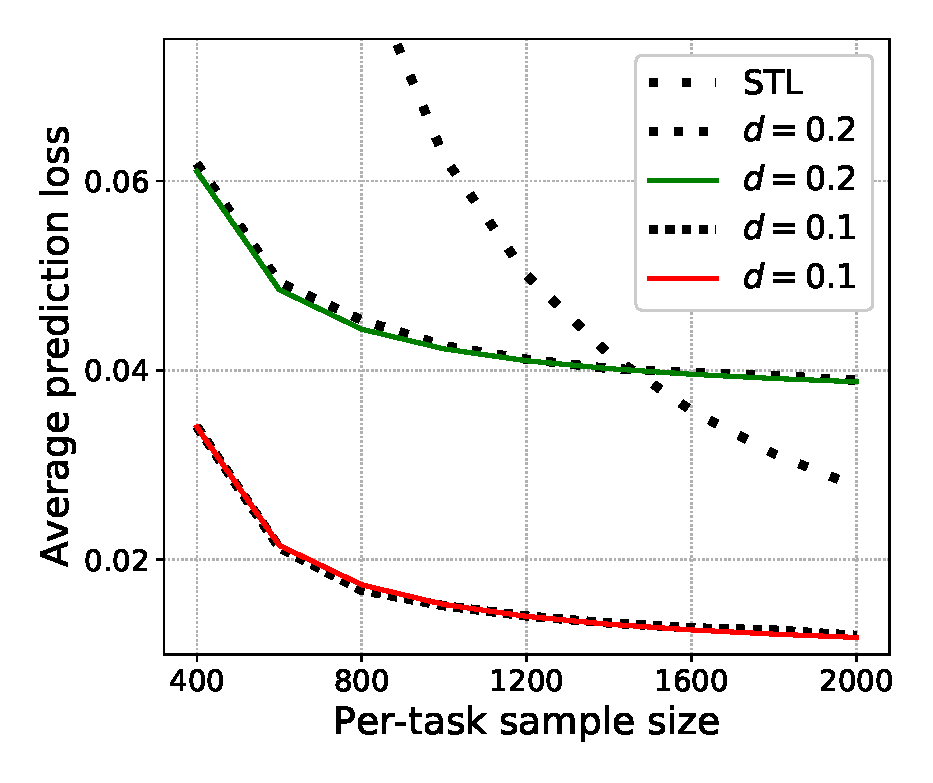
\includegraphics[width=0.9\textwidth]{figures/same_covariates.eps}
		\caption{Example \ref{ex_same_cov}}
		\label{fig_same_cov}
	\end{subfigure}\hfill
	\begin{subfigure}[b]{0.5\textwidth}
		\centering
		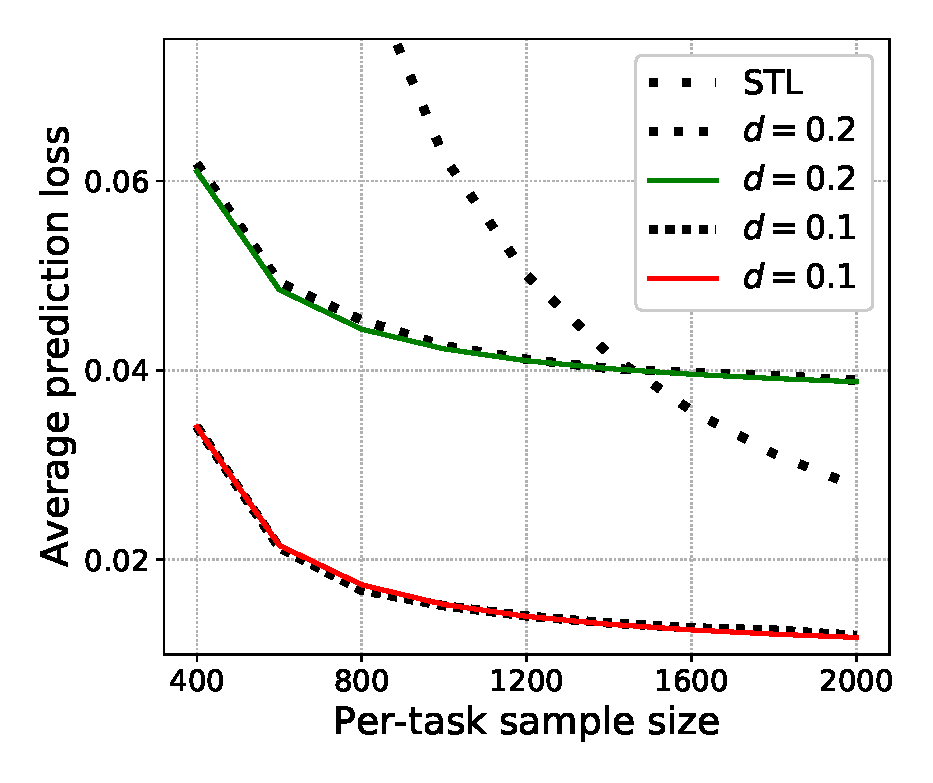
\includegraphics[width=0.9\textwidth]{figures/same_covariates.eps}
		\caption{Example \ref{ex_sample_ratio}}
		\label{fig_width}
	\end{subfigure}
%	\caption{%Three takeaways of our theory in Section \ref{sec_insight}.
%	Our estimated losses (solid line) match the empirical losses (dotted line) accurately under various settings in dimension $p = 200$.
%	\textbf{Left.} Validating Example \ref{ex_same_cov} for ten tasks: the noise variance $\sigma^2$ is $1/4$.
%	\textbf{Middle.} Validating Example \ref{ex_sample_ratio} for two tasks: we discover an interesting phenomena by fixing task two's sample size and increasing task one's sample size.
%	Moreover, our result accurately predicts the critical point (marked in circle) of the loss curve.
%	Depending on how large the distance $d^2$ is, task two's prediction loss decreases initially before increasing again, or decreases monotonically.
%	\textbf{Right.} We show how different levels of covariate shift affect hard parameter sharing when there is no bias.
%	Having covariate shift increases task two's prediction loss when task two's sample size is smaller than task one. Otherwise, having covariate shift (surprisingly) decreases task two's prediction loss.}
%	\label{fig_model_shift_phasetrans}
\end{figure*}

%Moreover, by setting $t=2$ in Theorem \ref{thm_many_tasks}, we can obtain the prediction loss for the HPS estimator for the transfer learning setting where the two tasks have the same covariates  $X^{(1)}=X^{(2)}$. For the reader's convenience, we give the precise statement in Corollary \ref{thm_two_tasks}.
%Theorem \ref{thm_many_tasks} implies Theorem \ref{thm_two_tasks} as a special case with $t=2$ and $r=1$.
%In this section, we consider the setting where the two tasks have the same covariates  $X^{(1)}=X^{(2)}$.
%We define $A^\star \in \R^{2}$ as the normalized eigenvector corresponding to the larger eigenvalue of the $2\times 2$ matrix
%$ {B^\star}^\top \Sigma  B^\star,$ where recall that $B^\star \define [{\beta}^{(1)},{\beta}^{(2)}] \in \real^{p\times 2}$ by definition.
% is the matrix formed by the linear model parameters of the two tasks.
%Without loss of generality, we assume that the two eigenvalues of ${B^\star}^\top \Sigma B^\star$ are not degenerate, so that $A^\star$ is uniquely defined. %Otherwise, Theorem \ref{thm_two_tasks} will give a null result.
%In the following corollary, the estimate \eqref{minimizer_beta1} shows that the minimizer $\hat a$ is approximately equal to $A^\star(1)/A^\star(2)$, while \eqref{Li_multi0} gives the exact asymptotic limit of $L_2(\hat{\beta}_2^{\MTL}(\hat a)) $, together with an explicit convergence rate that we believe to be sharp.

%\begin{corollary}\label{thm_two_tasks}
%Under Assumption \ref{assm_big1}, suppose that $X^{(1)}=X^{(2)}$ and $n_1=n_2\equiv n$. Let $c>0$ be an arbitrary (small) constant. Then we have that with high probability,
%\be\label{minimizer_beta1}
%\left\| u_{\hat a}u_{\hat a}^\top - A^\star {A^\star}^\top\right\|_F  \le  \left[\frac{ n^{-1/2+2/\varphi+c}  \|{B^{\star}}^{\top}\Sigma B^{\star}\|  + n^{-1/2+c} \sigma^2 }{\lambda_1 - \lambda_{2} } \right]^{1/2},
%\ee
%where $u_{\hat a}$ is the unit vector defined as
%$ u_{\hat a}:= \frac1{\hat a^2 +1} \begin{pmatrix} {\hat a}\\ %1\end{pmatrix},$ and $\lambda_1 $ and $\lambda_{2}$ are respectively the larger and smaller eigenvalues of ${B^\star}^\top\Sigma B^\star$.
%for task 2,  % over the randomness of the input,
%Moreover, the prediction loss of the HPS estimator satisfies that with high probability,
%	\begin{align}
%		& \bigabs{L_2(\hat{\beta}_2^{\MTL}(\hat a)) - \left\|(\Sigma^{(2)})^{1/2} \left(A^\star(2) \cdot B^{\star}A^{\star}  - \beta^{(2)}\right)\right\|^2  - |A^\star(2)|^2  \frac{p\sigma^2}{n-p} } \nonumber\\
%		& \le  \left[  \frac{  n^{-1/2+2/\varphi+c} \|{B^{\star}}^{\top}\Sigma B^{\star}\|+n^{-1/2+c} \sigma^2} {\lambda_1  - \lambda_2 }\right]^{1/2}   \left(\norm{\Sigma^{1/2} B^{\star}}^2+  \sigma^2\right), \label{Li_multi0}
		%\le n^{-\frac{c_{\varphi}}2} \cdot \frac{\bigbrace{ \norm{\Sigma^{1/2} B^{\star}}^2+  \sigma^2} \cdot (\bignormFro{\Sigma^{1/2} B^{\star}}^2 + \sigma^2 t)} {\lambda_r ({B^\star}^\top \Sigma B^\star)- \lambda_{r+1}({B^\star}^\top \Sigma B^\star)},
%	\end{align}
%	 where $A^\star(2)$ denotes the second entry of $A^\star$.
%	 \end{corollary}

\begin{example}[How to set the width $r$ in HPS?]
\label{ex_same_cov}
%Suppose every $\beta^{(i)}$ consists of two random components, one that is shared among all tasks and one that is task-specific.
%Thus, each task contributes a certain amount to the shared component and injects a task-specific bias.
%More precisely, %we have
An important question in applications of HPS is how to set the width $r$ of the feature layer.
We use our estimates to show that the optimal width depends on the tradeoff between the estimator's bias and variance.
Concretely, consider a random-effect model where all tasks share a model vector $\beta_0$ plus perturbations.
For every $i=1,2,\cdots, t,$, $\beta^{(i)} = \beta_0 + \wt \beta^{(i)}$, where $\wt \beta^{(i)}$ denotes the $i$-th task-specific component whose entries are i.i.d. Gaussian random variables of mean zero and variance $\frac {\kappa^2} p$.

\begin{claim}
\begin{enumerate}
	\item {\bf Positive vs. negative transfer.} The averaged HPS prediction loss is smaller than the single-task OLS prediction loss if and only if $\frac{d^2}{p}\tr \Sigma  < \frac{p\sigma^2 }{n - p}$, that is, the ``task-specific variance'' is smaller than the ``noise variance'' up to some constant factor.
	
	\item {\bf The optimal rank $r$.} If $\frac{d^2}{p}\tr \Sigma  < \frac{\sigma^2 p}{n - p}$, then the smallest averaged HPS  prediction loss is achieved when $r=1$. Hence increasing the width $r$ of the shared feature representation layer does not help.
\end{enumerate}
\end{claim}
%For our discussion below, we assume that $\kappa^2 \sim d^2 \sim \sigma^2$ and $n\sim p$. %and $d^2=\OO(\kappa^2)$.
%The more precise conditions on the relations between $d^2$, $\sigma^2$ and $\kappa^2$ are given in  \eqref{choiceofpara}.
%We assume that all the random variables have finite moments up to any order as in equation \eqref{assmAhigh2}.
\begin{proof}
    In this random-effect model, using the concentration of Gaussian random vectors (e.g. Lemma \ref{largedeviation} in the supplement  \cite{MTL_suppl}),
    %Based on the definition of the random-effect model,
    the $(i, j)$-th entry of ${B^{\star}}^{\top} \Sigma B^{\star}$ is equal to %(ignoring lower order terms)
    %\begin{align*}
    %	\beta_i^{\top} \beta_j \approx \norm{\beta_0}^2 + \frac{d^2}{2}\delta_{ij},\quad 1\le i,j \le t,
    %\end{align*}
    \begin{align}\label{betaSbeta}
    	\beta_i^{\top}\Sigma  \beta_j =\beta_0^\top \Sigma \beta_0 + \delta_{ij} \frac{d^2 }{p}\tr \Sigma + \OO\left(p^{-1/2+c}\|\beta_0\|^2+ p^{-1/2+c} d^2\right),
    \end{align}
     with high probability for any constant $c>0$. We omit the details to show the error bound using Lemma \ref{largedeviation}.
    %Note that $\norm{\beta_0}^2$ is approximately $\kappa^2$.
    With \eqref{betaSbeta}, it is easy to calculate that with high probability, the eigenvalues of ${B^{\star}}^{\top} \Sigma B^{\star}$ are given by
    $$\lambda_1=\left[1+\OO(p^{-1/2+c})\right]\cdot\left(t \beta_0^\top \Sigma \beta_0  + \frac{d^2}{ p}\tr \Sigma\right) ,$$
    and
    $$ \lambda_i=\left[1+\OO(p^{-1/2+c})\right]\cdot \frac{d^2}{ p}\tr \Sigma , \ \ i=2,\cdots, t.$$ %Therefore, by taking a rank-$1$ approximation of ${B^{\star}}^{\top} B^{\star}$, we get the average prediction loss of $B^{\star} a_i^{\star}$.
    Thus for the best rank-$r$ approximation $A^\star {A^\star}^\top$  of ${B^{\star}}^{\top}\Sigma  B^{\star}$, we have
    $$\bignorm{\Sigma^{1/2} B^{\star} (A^\star {A^\star}^{\top} - \id_{t\times t})}_F^2= [1+\OO(p^{-1/2+c})]\cdot(t-r)\frac{d^2}{ p}\tr \Sigma $$
    with high probability.
    %To see this, recall that $r$ is one and $A^{\star} {A^{\star}}^{\top}$ is the best rank-$1$ approximation of ${B^{\star}}^{\top}\Sigma B^{\star} = {B^{\star}}^{\top} B^{\star}$.
    %Hence, the above expression is equal to the sum of ${B^{\star}}^{\top} {B^{\star}}$'s bottom $t-1$ singular values.
    %In the random-effect model described above, we further assume that $\Sigma$ is isotropic as an example.
    %We show that when the rank $r$ is one, the average prediction loss of hard parameter sharing is as follows
    Then using \eqref{Li_multi2}, we obtain that
    \[ \frac{1}{t}\sum_{i=1}^t L_i(\hat{\beta}_i^{\MTL}) = \bigbrace{1 - \frac{r}{t}} \frac{d^2}{p}\tr \Sigma + \frac{r}{t} \cdot \frac{p\sigma^2 }{n - p} +\oo(\|\beta_0\|^2+d^2 + \sigma^2) ,\quad \text{w.h.p. }\]
    %We describe a proof sketch.
    %First, we show that the bias equation $L(B^{\star} a_i^{\star})$ simplifies to the following
    %\[ \frac{1}{t} \sum_{i=1}^t L(B^{\star} a_i^{\star}) = \frac{1}{t}\normFro{B^{\star} A^{\star} {A^{\star}}^{\top} - B^{\star}}^2 \approx \left(1 - \frac{1}{t}\right) {d^2}{}  . \]
    %Second, using Fact \ref{fact_tr}, one can see that the average variance is
    %\begin{align*}
    %	\frac{1}{t} \sum_{i=1}^t \sigma^2\norm{a_i^{\star}}^2 \bigtr{\Sigma (X^{\top} X)^{-1}} = \frac{\sigma^2}{t} \sum_{i=1}^t \norm{a_i^{\star}}^2 \frac{p}{n - p}
    %	= \frac{1}{t}\frac{\sigma^2 p}{n - p},
    %\end{align*}
    %because $A^{\star}$ has rank-$1$ and $\sum_{i=1}^t \norm{a_i^{\star}}^2 = 1$.
    %Combined together, we have derived the average prediction loss in the random-effect model.
    %If the error is sufficiently small, then
    %Recall that the average prediction loss of STL scales as $\sigma^2\cdot \bigtr{\Sigma (X^{\top} X)^{-1}} = \frac{\sigma^2 p}{n - p}$ by Fact \ref{fact_tr}.
    %Comparing HPS to STL, we have the following qualitative properties.
    %	Suppose $n$ is sufficiently large so that the error is negligible.
\end{proof}
\end{example}



%We demonstrate the accuracy of our results in simulations.
%While our theory is asymptotic (with error terms that are negligible when $p$ is sufficiently large), we observe that they are incredibly accurate in a moderate dimension of $p = 200$.



First, we validate the result of Example \ref{ex_same_cov}.
Figure \ref{fig_same_cov} shows the average prediction loss over ten tasks as we increase the number of samples per-task from $400$ to $2000$.
In all the parameter settings, our results estimate the empirical losses accurately.
We also observe a trend that the average prediction loss increases as we increase distance $d$ from $0.1$ to $0.2$.
Our work explains the differences between these two settings since $d^2 = 0.1^2$ is always smaller than $\frac{\sigma^2 p}{n - p}$, but $d^2 = 0.2^2$ is not.
%Second, when $d = 0.1$, we have that $d^2 \le \frac{\sigma^2 p}{n - p}$ for all values of $n$, hence the average prediction loss of hard parameter sharing is always lower than STL.
Indeed, we observe a crossover point between hard parameter sharing and STL.
Finally, for $d = 0.2$, looking horizontally, we find that HPS requires fewer samples per-task than STL to achieve the same loss level. %\FY{I do not quite understand this sentence about "3x fewer", because how much data needed depends on $d$ and the prediction loss level we are looking at. For example, at the cross point, this ratio is 1. }


%Our result from Corollary \ref{cor_MTL_loss} explains this trend.


%Covariate shift: We set $\kappa = 1$ and $d = 0$.
%We set $\rho_2 = 4$ and vary $\rho_1$ from $5$ to $25$ for sample sizes.
%We use the scale parameter $\lambda = 1$ for the curve without covariate shift and $\lambda = 2$ for the curve with covariate shift (cf. Section \ref{sec_covshift}).


%Recall that Section \ref{sec_data_size} shows that increasing the data size of the source task does not always improve the performance of MTL for the target task.
%In Figure \ref{fig_ab_data}, we show that for source task MR and target task SST, there is a transition from positive to negative transfer as we increase the data size of the source task.
%Our result provides a fine-grained insight on the covariance alignment algorithm proposed in \cite{WZR20}.
%Recall that the covariance alignment procedure in \cite{WZR20} adds an additional module between the word embedding representation and the shared module.
%When the source task data size is particularly large compared to the target task, we show that applying the covariance alignment algorithm results in more significant gains.
%In Figure \ref{fig_ab_cov}, we observe that the benefit from aligning task covariances becomes more significant for LSTM and MLP as we increase the number of datapoints of the source task.

%\begin{table}
%	\begin{center}
%		\begin{tabular}{c c c c c}
%			\toprule
%			\multirow{2}{*}{{\bf Models}} & \multicolumn{2}{c}{\begin{minipage}{1.1in}\begin{center}
%				                                                                          MR, SST, SUBJ, CR, MPQA, TREC\end{center}\end{minipage}} & \multicolumn{2}{c}{\begin{minipage}{1.1in}\begin{center}MR, SST, SUBJ, CR, MPQA\end{center}\end{minipage}} \\
%			\cmidrule(lr){2-3} \cmidrule(lr){4-5}
%			& {\bf Stanford} & {\bf Alignment} & {\bf Stanford} & {\bf Alignment} \\
%			\midrule
%			{\bf MLP}  & > 100\% & 39\% & 25\% & 25\% \\
%			{\bf LSTM} & 36\% & 36\% & 28\% & 25\% \\
			% {\bf CNN}  & 76\% & - & 32\% & -\\
%			\bottomrule
%		\end{tabular}
%	\end{center}
%	\caption{Taskonomy experiment.}
%	\label{tab:taskonomy}
%\end{table}
%\begin{figure}[!t]
%	\centering
%	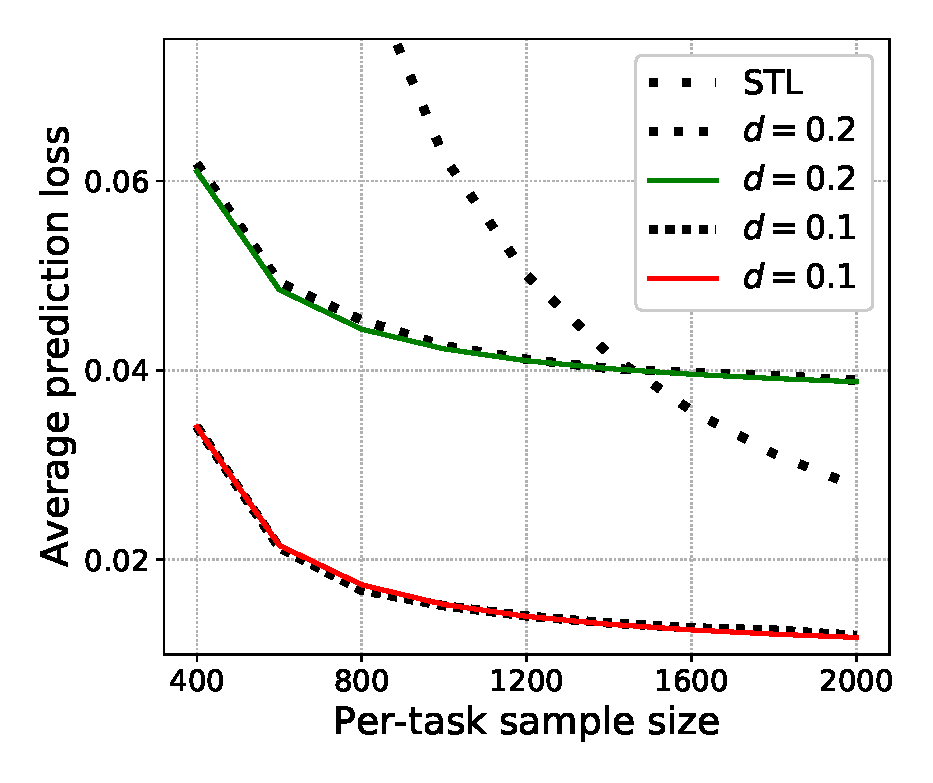
\includegraphics[width=0.35\textwidth]{figures/same_covariates.eps}
%	\caption{Validating Example \ref{ex_same_cov} in Section \ref{sec_same} for $10$ tasks: our estimated loss (solid line) matches the empirical loss (dotted line) accurately for various task-specific variance $d^2$ and sample size $n$ settings. The feature dimension $p$ is $200$, and noise variance $\sigma^2$ is $1/4$.}
%	\label{fig_same_cov}
%\end{figure}





%The estimate \eqref{minimizer_beta1} shows that the minimizer $\hat a$ is approximately equal to $A^\star(1)/A^\star(2)$, while \eqref{Li_multi0} gives the exact asymptotic limit of $L_2(\hat{\beta}_2^{\MTL}(\hat a)) $, together with an explicit convergence rate that we believe to be sharp.


%It is not hard to extend the above result to the cases with more than two tasks. We make this extension for the following reasons. First, it provides a clearer geometric intuition than the two-task setting as we will discuss below. Second, the corresponding multi-task setting is prevalent in applications of multi-task learning to image classification, where there are multiple prediction labels/tasks for every image \cite{chexnet17,EA20}. Finally, it provides useful insights into a more general theory of multi-task learning, which we will explore in greater details in future works.

%We consider an arbitrary local minimum $B, W_1, \dots, W_2$ of the optimization objective.
%We extend the bias-variance decomposition from the two-task case to the multiple-task case.
%We observe that the expected prediction loss of $\hat{\beta}_t^{\MTL}$ conditional on $X$ consists of a bias and a variance equation as follows
%\begin{align}
%	\exarg{\varepsilon_1, \dots, \varepsilon_t}{L(\hat{\beta}_t^{\MTL}) \mid X}
%	=& \bignorm{\Sigma^{1/2} \bigbrace{B^{\star} \cW^{\top} (\cW \cW^{\top})^{-1} W_t - \beta_t}}^2 \label{eq_bias_multiple} \\
%	&+ \sigma^2 \cdot (W_t^{\top} (\cW \cW^{\top})^{-1} W_t) \cdot \bigtr{\Sigma (X^{\top} X)^{-1}} \label{eq_var_multiple}
%\end{align}
%One can see that equation \eqref{eq_bias_multiple} is the bias of the multi-task learning estimator and equation \eqref{eq_var_multiple} is its variance.
%Compared to the prediction loss of single-task learning (cf. equation \eqref{eq_var_stl}), we observe that the variance equation \eqref{eq_var_multiple} is always smaller because $W_t^{\top} (\cW \cW^{\top})^{-1} W_t \le 1$.
%On the other hand, the bias equation \eqref{eq_bias_multiple} is always larger because of the difference between the task models.
%We show the generalization error of hard parameter sharing estimators.
%Before stating the result, we define the following notations.




%The key step for proving Theorem \ref{thm_many_tasks} is a characterization of $f(A, B)$'s global minimizer.
%\medskip
%
%\noindent\textbf{Comparison to single-task learning (STL).}
%Theorem \ref{thm_many_tasks} provides a sharp generalization error bound that is asymptotically tight when $n$ goes to infinity.
%%The limiting loss of hard parameter sharing consists of two parts, a bias term $L(B^{\star} a_i^{\star})$ that measures the error of $B^{\star} a_i^{\star}$, and a variance term that scales with noise variance $\sigma^2$.
%%	Our result implies that the variance of hard parameter sharing is always smaller than single-task learning.
%%	This is because	STL's variance is equal to $\frac{\sigma^2 \cdot p} {n - p}$ by Fact \ref{lem_minv}, and $\norm{a_i^{\star}}^2 \le 1$ since the spectral norm of $U_r$, which is a projection matrix, is at most one.
%One direct implication of our result is that compared to STL, the variance always decreases, since STL's variance is equal to $\sigma^2 \tr[\Sigma (X^{\top} X)^{-1}]$.
%On the other hand, the bias always increases.


%\FY{add simulations to check our results; discuss motivations and possible applications}
\iffalse
In this paper, we consider a natural extension of the estimator $\hat \beta^{\rm{TL}} $, that is, the \emph{hard parameter sharing} (HPS) estimator, which has been a standard type of estimator in multi-task learning \FY{citations}. More precisely, we study the following HPS architecture: a shared feature representation layer $B\in\real^{p}$ for all datasets and a separate output layer $A_i \in \real$ for every dataset $i$. Then we study the following minimization problem:
\begin{align}\label{eq_tsl}
			f(A, B) = \norm{X^{(1)} B A_1 - Y^{(1)}}^2 + \norm{X^{(2)} B A_2 - Y^{(2)}}^2,
\end{align}
where we abbreviate $A = [A_1, A_2]$. Let $(\hat{A}, \hat{B})$ be the minimizer of $f(A, B)$. We define the hard parameter sharing (HPS) estimator for task $i$ as
\be\label{def_HPS}\hat{\beta}_i^{\MTL} = \hat{B} \hat{A}_i,\quad i=1,2.\ee
Note that $\hat \beta^{\rm{TL}}$ is a special case of $\hat{\beta}_i^{\MTL}$ by setting $A_1=A_2=1$.

For the optimization objective $f(A, B)$ in \eqref{eq_tsl}, using the local optimality condition $\frac{\partial f}{\partial B} = 0$, we can solve that
	\begin{align}
		\hat{B} = A_2^{-1} \hat \Sigma(a)^{-1} \left[a (X^{(1))})^{\top}Y^{(1)} +  (X^{(2)})^{\top}Y^{(2)}\right], \label{eq_Bhat_2task} %\\
		%&= (B^\star A ^{\top}) (A A^{\top})^{-1} + (X^{\top}X)^{-1}X^{\top}   \bigbrace{\sum_{j=1}^t \varepsilon_i A_i^{\top}} (A  A^{\top})^{-1}.
	\end{align}
where we denote $a:=A_1/A_2$ and $\hat \Sigma(a):= a^2 (X^{(1)})^\top X^{(1)}  + (X^{(2)})^\top X^{(2)}$.
Applying $\hat B$ to equation \eqref{eq_tsl}, we obtain an objective that only depends on $a $ as follows %\HZ{$A$ has been used to denote the output layers. Could you replace $A$ with another symbol (say $x$)?}
 \begin{align}
		 g(a) \define & \left\| X^{(1)} \hat\Sigma(a)^{-1} (X^{(2)})^\top X^{(2)} (a\beta^{(2)}-\beta^{(1)}) \right. \nonumber\\
			& \left. + \left(a^2 X^{(1)}\hat \Sigma(a)^{-1} (X^{(1)})^\top-\id_{n_1\times n_1}\right)\epsilon^{(1)}+ a X^{(1)}\hat \Sigma(a)^{-1} (X^{(2)})^\top \epsilon^{(2)} \right\|^2 \nonumber\\
		   +& \left\| X^{(2)} \hat \Sigma(a)^{-1} (X^{(1)})^\top X^{(1)} (a\beta^{(1)}-a^2\beta^{(2)}) \right. \nonumber\\
		  &\left.+ \left(X^{(2)}\hat\Sigma(a)^{-1} (X^{(2)})^\top-\id_{n_2\times n_2}\right)\epsilon^{(2)} + a X^{(2)}\hat \Sigma(a)^{-1} (X^{(1)})^\top \epsilon^{(1)} \right\|^2. \label{eq_mtl_A12}
	\end{align}
Let $\hat a$ be the minimizer of $g(a)$. Throughout this paper, we regard $Y^{(1)}$ as the source data, and $Y^{(2)}$ as the target data.  Then the HPS estimator \eqref{def_HPS} for the target task 2 is
\be\label{HPS_est}
\hat{\beta}_2^{\MTL} (\hat a) = \hat \Sigma(\hat a)^{-1}  \left[\hat a (X^{(1))})^{\top}Y^{(1)} +  (X^{(2)})^{\top}Y^{(2)}\right].
\ee
\fi




\section{Discussions}\label{sec_conclude}
\FY{Conclusions are not needed for AOS. If you want to have this section, please use it to give some additional remarks that are not discussed yet, and to discuss about possible futuer works.}
This work studied generalization properties of a widely used hard parameter sharing approach for multi-task learning.
We provided sharp bias-variance tradeoffs of HPS in high-dimensional linear regression.
Using these results, we analyzed how varying sample sizes and covariate shifts impact HPS, and rigorously explained several empirical phenomena such as negative transfer and covariate shift related to these dataset properties.
We validated our theory and conducted further studies on text classification tasks.
We describe several open questions for future work.
%First, it would be interesting to tighten our estimate in Corollary \ref{cor_MTL_loss}, which would extend the observation in Figure \ref{fig_size} to small $n_1$.
%Second, it would be interesting to extend our result to classification problems such as logistic regression.
First, our result in Corollary \ref{cor_MTL_loss} involves an error term that scales down with $n_1$.
Tightening this error bound requires showing the limit of $\normFro{({Z^{(1)}}^{\top} Z^{(1)} + {Z^{(2)}}^{\top} Z^{(2)})^{-1} {Z^{(1)}}^{\top} Z^{(1)}}^2$ for two isotropic sample covariance matrices.
This requires studying the asymptotic singular values distribution of the non-symmetric matrix $({Z^{(1)}}^{\top} Z^{(1)})^{-1}{Z^{(2)}}^{\top} Z^{(2)}+\id$, which is still an open problem in random matrix theory.
%FY: $+\id$ is very important and makes the problem very hard; otherwise the problem can be solved with current RMT methods.
The eigenvalue distribution of this matrix, which has been obtained in \cite{Fmatrix}, might be helpful towards resolving this problem.
%but its singular values will follow a different distribution since the matrix is not symmetric.
 %might require new techniques beyond the current ones in random matrix theory .%\HZ{to add}.
Second, it would be interesting to extend our results to classification problems.
Several recent work have made remarkable progress for logistic regression in the high-dimensional setting, e.g. \cite{sur2019modern}.
An interesting question is to study logistic regression in a multiple-sample setting.


\begin{supplement}
\textbf{Supplement to ``High-dimensional Asymptotics of Information Transfer for Linear Regression under Covariate Shifts"}.
In the Internet Appendix \cite{MTL_suppl}, we provide the proofs of the technical results in Sections \ref{sec_HPS}-\ref{sec_diff}, including Lemma \ref{lem_HPS_loss}, Theorem \ref{thm_many_tasks}, Theorem \ref{cor_MTL_loss}, Proposition \ref{lem_hat_v}, Theorem \ref{thm_main_RMT} and Proposition \ref{prop_main_RMT}.
%and give the technical proofs of the main theorems, Theorems \ref{thm_regularbm}, \ref{thm_twgram}, \ref{thm_twgraph} and  \ref{thm_twgraph_sparse}.
\end{supplement}



\bibliographystyle{imsart-number}
\bibliography{rf,ref_mtl}

\end{document}
